\documentclass[12pt]{article}
\usepackage{afterpage}
\usepackage{array}
\usepackage{cite}
\usepackage{float}
\usepackage{glossaries}
\usepackage{graphicx}
\usepackage{hyperref}
\usepackage{listings}
\usepackage{mathptmx}
\usepackage{multicol}
\usepackage{qrcode}
\usepackage{textcomp}

\usepackage[a4paper,
            left=1in,
            right=1in,
            top=1in,
            bottom=1in,
            footskip=.5in]{geometry}

\newcommand\blankpage{
    \null
    \thispagestyle{empty}
    \addtocounter{page}{-1}
    \newpage}

\makeglossaries
\loadglsentries{definitions}

\begin{document}

% Front page:
\begin{titlepage}
    \begin{center}
        {\Large Faculty of Electrical and Computer Engineering}

        {\Large Laboratory for Control Robotics and Machine Learning}

        \vspace{1cm}
        
        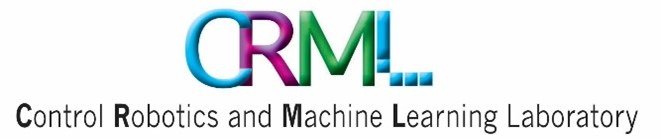
\includegraphics[width=0.5\textwidth]{images/CRML_logo.jpg}
        
\includegraphics[width=0.4\textwidth]{images/Technion_logo.png}

        \vspace{1.5cm}

        Subject:

        \vspace{0.3cm}
        
        \textbf{\Huge Optimal Path Planning for a Robot in an Unknown Environment}
            
        \vspace{1.5cm}

        Authors:
        
        \vspace{0.3cm}
        
        {\Large
            Omer Huly
            \&
            Roy Abudi}

        \vspace{1cm}

        Supervisor:

        \vspace{0.3cm}
        
        {\Large Mr. Ori Menashe}

        \vspace{1cm}

        Semester:

        \vspace{0.3cm}
        
       {\Large Winter 2024}        
    \end{center}
\end{titlepage}

\blankpage

\tableofcontents

\newpage

\addcontentsline{toc}{section}{List of Tables and Figures}
\listoffigures
\listoftables
\lstlistoflistings

\newpage

\section{Abstract}
The \gls{Micromouse} competition has been running since the late 1970s around the world.
The goal is simple: get to the end of the \gls{maze} as fast as possible.
To solve the problem, a simulation was built to visualize several algorithms' results.
The proposed solution combines several algorithms to ensure the robot can find the fastest route.
First, a flood-fill algorithm is used for mapping the \gls{maze}. The robot starts by trying to reach the goal and mapping the \gls{cell}s it encounters.
After that, it spends time searching for areas it did not visit, prioritizing large unexplored areas while avoiding dead-ends before returning to where it started.
After mapping the \gls{maze}, Dijkstra's algorithm is used to find the fastest route.
Although the flood-fill algorithm, which is very popular among \gls{Micromouse} competitors, can quickly find the shortest path from the start to the goal, using it alone does not guarantee finding the fastest route.
The proposed solution reinforces the flood-fill algorithm and helps solve the problem of finding the fastest route with greater accuracy.

\newpage

% This is the glossary.
% To add words to it, use \gls{word} and add a definition in the definitions file.
\printglossary

\newpage

\section{Introduction} \label{introduction}
\paragraph{}
Today, robots are used more and more. Often, robots should move or walk and find their path autonomously.
Therefore, the ability of robots to find their way around obstacles is needed.
This project is based on the \gls{Micromouse} competition as a basis for developing optimal path-planning algorithms in an unknown environment.
Each competition complies with the \gls{IEEE} \gls{Micromouse} standard rules.
The \gls{Micromouse} competition features small autonomous robots called "micromouse".
The task is to solve the \gls{maze}.
To complete this task, the robot needs to move from the start point to the final destination point in the center of the \gls{maze}.
The robot has no prior knowledge of the \gls{maze}.
The competition requires overcoming the engineering challenge of designing and programming a robot capable of solving the \gls{maze} as fast as possible.
Our project focuses on the algorithmic aspect of the problem and does not include a physical robot.
A simulation has been built to emulate the physical \gls{maze} environment and test our algorithms.

The competition is not new and there have been numerous attempts at solving the problem and refining the algorithms.
The na\"{i}ve wall-following algorithms were successful in the early days of the competition.
Later, the goal of the \gls{maze} was moved away from the edges.
This change could lead to a robot using a na\"{i}ve wall-following algorithm getting stuck in an infinite loop circling the \gls{maze} \cite{4725791}.
Later, more sophisticated algorithms were tested such as \gls{BFS} and \gls{DFS} for traversing the \gls{maze} but the former can be very slow because of backtracking and the latter is not guaranteed to find the fastest path.
The solving algorithm continued to develop over the years and today the most common algorithm used in \gls{Micromouse} is the flood-fill algorithm \cite{4725791}.
We will delve deeper into this algorithm and more later in this work.

In this paper, first, there will be an explanation of how the problem has been modeled.
After that, there will be an overview of the \gls{maze} simulation and its features.
Next, there will be a comprehensive review of the various algorithms that have been tested.
In section \ref{naive-algorithms}, na\"{i}ve algorithms such as random path and wall follower are discussed.
In section \ref{sophisticated-algorithms}, more sophisticated algorithms such as the flood fill algorithm and Dijkstra's algorithm are discussed.
Later in section \ref{new-algorithm}, an explanation of the main product, our new proposed algorithm is presented.
Finally, the results and conclusions are given in section \ref{results}.

\section{Modeling the Problem}
\subsection{Maze Structure and Rules}
% Wall rules, goals rules, starting point rules
% Some definitions - north, east, south, west
%    west v
%         +---+ < north
%         |   |
% south > +---+
%             ^ east
\paragraph{}
The \gls{maze} in the \gls{Micromouse} competition consists of a $16 \times 16$ grid of unit squares.
Each one of these squares is called a \gls{cell}.
External walls enclose the entire \gls{maze}.
The starting \gls{cell} of the \gls{maze} is located at one of the four corners and is always bounded by walls on three of its four sides.
The goal \gls{cell}s are a $2 \times 2$ square at the center of the \gls{maze} bounded by walls except for one opening.
The robot's objective is to achieve the shortest runtime.
A run begins every time the robot leaves the starting \gls{cell}.
When the robot reaches the goal, a runtime is recorded.
If the robot re-enters the starting \gls{cell}, the run ends, and a new runtime will begin when the robot leaves the starting \gls{cell}.
More about the competition rules can be found in section \ref{Competition Rules}.

Each \gls{cell}'s wall is represented by its absolute position around the edges of the \gls{cell}.
Therefore, the wall on the upper edge is referred to as the north wall.
The wall on the left edge is referred to as the east wall.
The wall on the lower edge is referred to as the south wall.
Lastly, the wall on the right edge is referred to as the west wall.
Figure \ref{cell figure} presents a \gls{cell} and its walls for clarity.

\begin{figure}[H]
\centering
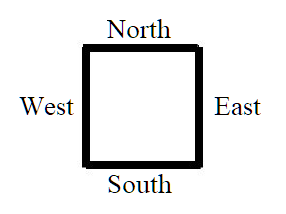
\includegraphics[width=0.3\textwidth]{images/cell_walls.png}
\caption{The name of each wall surrounding a \gls{cell}}
\label{cell figure}
\end{figure}

A \gls{maze} is considered valid if it is: 
\begin{enumerate}
    \item Non-empty
    \item Rectangular
    \item Enclosed - all outer walls of the \gls{cell}s on the perimeter of the \gls{maze} are present.
    \item Consistent - adjacent \gls{cell}s agree on their shared wall.
\end{enumerate}

\subsection{Maze Representation}
\subsubsection{Prologue}
\paragraph{}
There are many possible ways to represent a \gls{maze}.
This section gives an overview of the different \gls{maze} representations we found that are used in previous works about the \gls{Micromouse} challenge \cite{AD-Codex-Micromouse-C-Simulation-2022, jimenezjose-Micromouse-Simulator, mackorone-mms, vineetvb-micromouse}.
The various \gls{maze} representations are named after the most common file suffix for \gls{maze} files using them.
Later, in section \ref{Chosen Maze Representation}, the chosen representation, which is used for the simulation and mapping of the \gls{maze} by the robot's algorithm, will be explained.

\subsubsection{"maz" Format Representation} \label{maz-format}
% Our memory representation [C++/C implementations]
% Nicest and simplest in memory <- This is the reason we chose this
\paragraph{}
Each \gls{cell} is represented by its four walls using a single bit per wall where '1' represents an existing wall and '0' represents a missing wall.
The memory layout of a \gls{cell} is described in the following table.

\begin{table}[H]
    \centering
    \begin{tabular}{ |c|c|c|c|c|c|c|c|c| }
    \hline
        bit & 7 & 6 & 5 & 4 & 3 & 2 & 1 & 0\\
    \hline
        value & 0 & 0 & 0 & 0 & W & S & E & N\\
    \hline
    \end{tabular}
    \caption{"maz" format \gls{cell} memory layout}
    \label{maz format cell memory}
\end{table}

The lower \gls{nibble} is where the wall's data resides.
The letters $N$, $E$, $S$, and $W$ represent the North, East, South, and West walls respectively.
The upper \gls{nibble} is ignored.
Thus, the whole \gls{maze} is represented by a two-dimensional array of \gls{cell}s where the index of each \gls{cell} is the coordinate of that \gls{cell} in the \gls{maze}.
The top left \gls{cell} in the \gls{maze} has a coordinate of $(0, 0)$.
An example of this format and the resulting \gls{maze}:

\vbox{
\begin{multicols}{2}
File (hex):
\begin{lstlisting}
    09 03 0b 0e 0c 06
\end{lstlisting}
\vfill\null
\columnbreak

Result:
\begin{lstlisting}
    +---+---+---+
    |       |   |
    +   +   +   +
    |   |       |
    +---+---+---+
\end{lstlisting}
\end{multicols}
}

\subsubsection{"CSV" Format Representation}
% The Ridiculous 1-16 non-bitmap representation [C in .cpp implementations]
% Mentioned and supported because although it's ridiculous, it is widely used.
\paragraph{}
A text format based on the \gls{CSV} file format.
Each row contains integers separated by commas.
The coordinate of the \gls{cell} in the \gls{maze} is determined by its position in the text.
The first integer in the first row is the top left corner of the \gls{maze}.
The next integer in the first row is the \gls{cell} to the right of the first one.
The first integer in the second row is the \gls{cell} below the first integer in the first row.
And the pattern continues.
The integers are in the range $[1, 16]$.
Each integer represents a different wall combination around the \gls{cell} as can be seen in the following figure.

\begin{figure}[H]
\centering
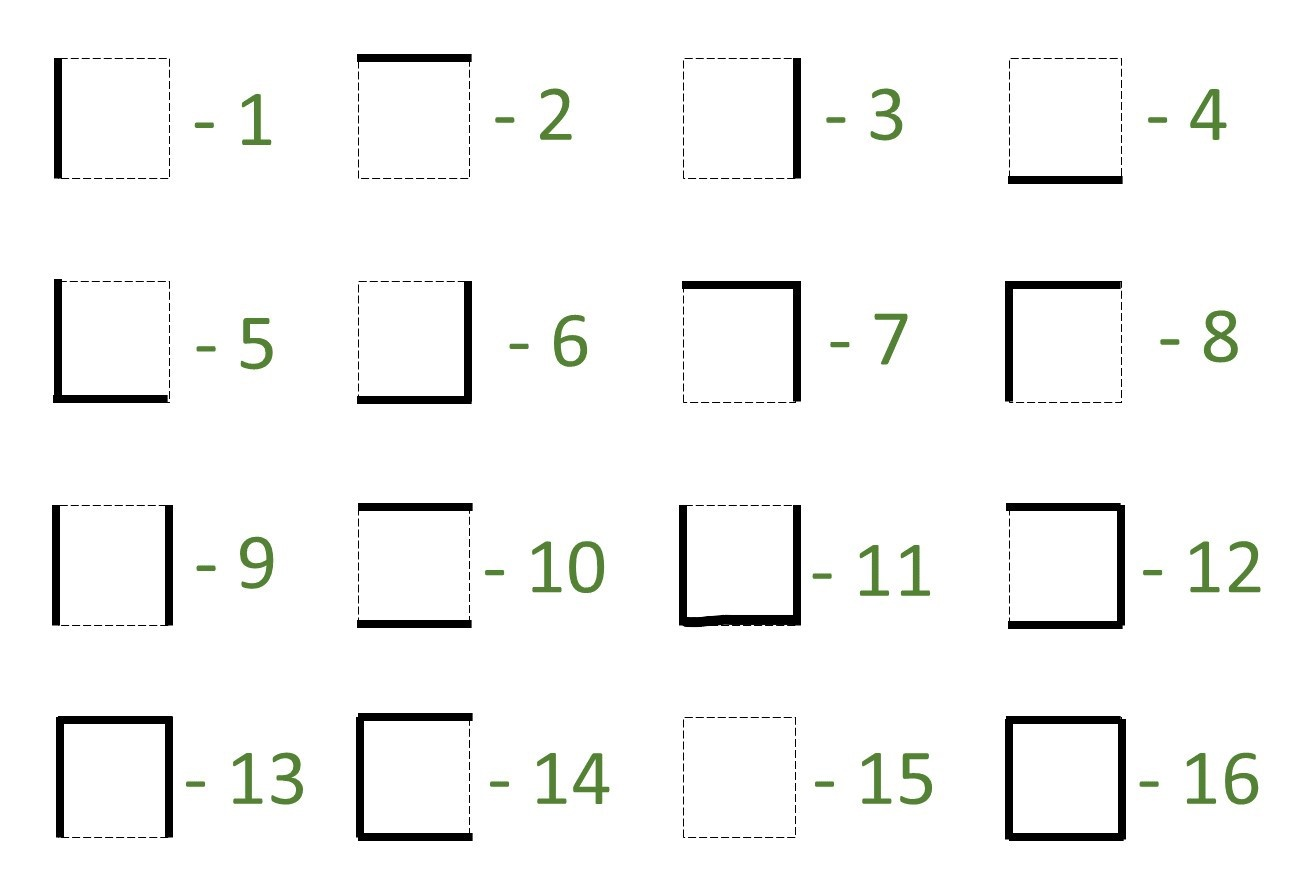
\includegraphics[width=0.6\textwidth]{images/CSV_format_diagram.png}
\caption{States for cell's walls in "CSV" format}
\end{figure}

The \gls{maze} starts empty, then for every line:
\begin{enumerate}
    \item The next integer is read and parsed.
    \item A \gls{cell} is created in the \gls{maze} at the corresponding coordinate.
    \item The new \gls{cell} is added with walls surrounding it based on the values of the integer.
\end{enumerate}
After all lines have been parsed, the \gls{maze} is checked for validity.
An example of this format and the resulting \gls{maze}:

\vbox{
\begin{multicols}{2}
File:
\begin{lstlisting}
    8, 7, 13
    11, 5, 6
\end{lstlisting}
\vfill\null
\columnbreak

Result:
\begin{lstlisting}
    +---+---+---+
    |       |   |
    +   +   +   +
    |   |       |
    +---+---+---+
\end{lstlisting}
\end{multicols}
}

\subsubsection{"num" Format Representation}
% The numbers for "x y n e w s" strange text format [C++ implementation with numbers inside]
% Worst format by far (in my opinion), from the same repository as the nice ASCII format so it was also included. Mostly to take maze files from there because that's what they used as the default.
\paragraph{}
A simple text format where each line is made up of 2 integer values, $X$ $Y$, followed by 4 boolean values, $N$ $E$ $S$ $W$, representing:
\begin{itemize}
    \item $X$, $Y$ - the \gls{cell}'s $X$ and $Y$ coordinates.
    $X$ is the horizontal axis (columns), $Y$ is the vertical axis (rows), and $(0, 0)$ is the bottom left corner.
    \item $N$, $E$, $S$, $W$ - North, East, South, West - represent where the \gls{cell} has walls.
\end{itemize}
The \gls{maze} starts empty, then for every line:
\begin{enumerate}
    \item The numbers are read and parsed.
    \item A \gls{cell} is created in the \gls{maze} at the $(X, Y)$ coordinate.
    \item The new \gls{cell} is added with walls surrounding it based on the values of $N$, $E$, $S$, and $W$.
\end{enumerate}
After all lines have been parsed, the \gls{maze} is checked for validity.
An example of this format and the resulting \gls{maze}:

\vbox{
\begin{multicols}{2}
File:
\begin{lstlisting}
    0 0 0 1 1 1
    0 1 1 0 0 1
    1 0 0 0 1 1
    1 1 1 1 0 0
    2 0 0 1 1 0
    2 1 1 1 0 1
\end{lstlisting}
\vfill\null
\columnbreak

Result:
\begin{lstlisting}
    +---+---+---+
    |       |   |
    +   +   +   +
    |   |       |
    +---+---+---+
\end{lstlisting}
\end{multicols}
}

\subsubsection{"maze" Format Representation} \label{maze-format}
% Our ".maze" file [C++ implementation with numbers inside, same repo as "num"]
% The only graphical one <- This is the reason we use this in files and for printing
\paragraph{}
A simple \gls{ASCII} file containing the \gls{maze} itself.
\gls{cell}s are 5 characters wide and 3 characters long and have a shared wall with each adjacent \gls{cell}.
The \gls{maze} starts empty.
The height and width of the \gls{maze} are calculated.
Then, for each \gls{cell} a wall is set if there wasn't a space in its location.
After that, the \gls{maze} is checked for validity.
An example of this format:

\def\simpleMazeMargin{52mm}

\vbox{
\begin{center}
File:
\lstset{
  xleftmargin=\simpleMazeMargin,
  xrightmargin=\simpleMazeMargin
}
\begin{lstlisting}
    +---+---+---+
    |       |   |
    +   +   +   +
    |   |       |
    +---+---+---+
\end{lstlisting}
\end{center}
}

\subsubsection{Chosen Maze Representation} \label{Chosen Maze Representation}
\paragraph{}
The "maz" representation defined in section \ref{maz-format} is used for the robot's in-memory \gls{maze} due to its simplicity and compatibility with basic bit-wise operations.
However, for ease of use, the "maze" representation defined in section \ref{maze-format} is used as the default for \gls{maze} input/output due to its visual nature.
However, our project supports input in all formats discussed above, which are then converted into the "maz" format representation.
We chose to support all formats to be able to use \gls{maze} input from all the sources we found \cite{AD-Codex-Micromouse-C-Simulation-2022, jimenezjose-Micromouse-Simulator, mackorone-mms, vineetvb-micromouse}.

\subsection{Robot Representation}
\paragraph{}
The robot is represented by a circle with a colored notch that illustrates the direction in which the robot is facing.
The robot occupies a single \gls{cell} in the \gls{maze}.
The robot can perform six types of actions:
\begin{enumerate}
    \item Ready to start
    \item Reset the algorithm and get back to the starting \gls{cell}
    \item Move forward one \gls{cell}
    \item Move backwards one \gls{cell}
    \item Rotate by 90\textdegree\ to the left
    \item Rotate by 90\textdegree\ to the right
\end{enumerate}

\section{Simulation}
\subsection{Overview}
\paragraph{}
The \gls{maze} simulation is designed to simulate and examine the algorithms while providing visual information about the execution process.
In addition, the simulation provides an interface between the robot and the \gls{maze}.
The simulation includes algorithms to choose from to solve the \gls{maze}.
Some of those algorithms are:
\begin{enumerate}
    \item Random - explained in section \ref{Random Algorithm}
    \item Left/Right wall-follower - explained in section \ref{Wall Following Algorithm}
    \item Flood-fill - explained in section \ref{Flood-Fill Algorithm}
    \item Flood-fill + Dijkstra - explained in section \ref{Combining Flood-Fill with Dijkstra's Algorithm}
    \item Thorough flood-fill - explained in section \ref{thorough flood-fill algorithm}
\end{enumerate}

In addition, an "idle" robot is provided for a robot that does nothing.
Of course, this robot can't solve a \gls{maze}.

\subsection{Robot-Maze Interaction}
\paragraph{}
The simulation works in "steps".
At each step, the simulation provides the robot with information about the walls of the \gls{cell} it is currently in.
Given this information, the robot decides what action to take and informs the simulation about it.
Next, the simulation ensures that the robot performed a legal action.
For example, if the robot is attempting to move forward one \gls{cell} while there is a wall right in front of it, the simulation will give an error and halt the execution of the algorithm.
If all checks are passed, the simulation updates the robot's position or orientation based on the action.
And the cycle repeats itself.
When the algorithm is finished, meaning the robot does not take any action, the simulation stops the execution.

\subsection{Graphical User Interface}
% \paragraph{}
% When the simulation starts, the simulation screen as seen in figure \ref{Simulation screen} is displayed.
% The simulation's controls can be found at the top of the screen as seen in figure \ref{Simulation controls close-up}.

% When the simulation starts, a screen that looks similar to figure \ref{Simulation screen} is displayed.
% A close-up of the simulation's controls can be seen in figure \ref{Simulation controls close-up}.
% A close-up of information about the exploration of the maze can be seen in figure \ref{Simulation bottom close-up}.

\paragraph{}
When the simulation starts, the simulation's screen as seen in figure \ref{Simulation screen} is displayed.
It includes the two main components in the simulation's screen:
\begin{itemize}
    \item A full \gls{maze} view that shows the robot, goal, and the fastest route calculated using Dijkstra's algorithm. Using Dijkstra's algorithm to find the fastest route in a \gls{maze} is expanded upon in section \ref{Dijkstra's Algorithm}.
    \item The robot's view - the \gls{maze} as seen by the robot. At the start of the simulation, the only known information is the starting \gls{cell}'s walls and the goal \gls{cell}s' location.
\end{itemize}

\begin{figure}[H]
\centering
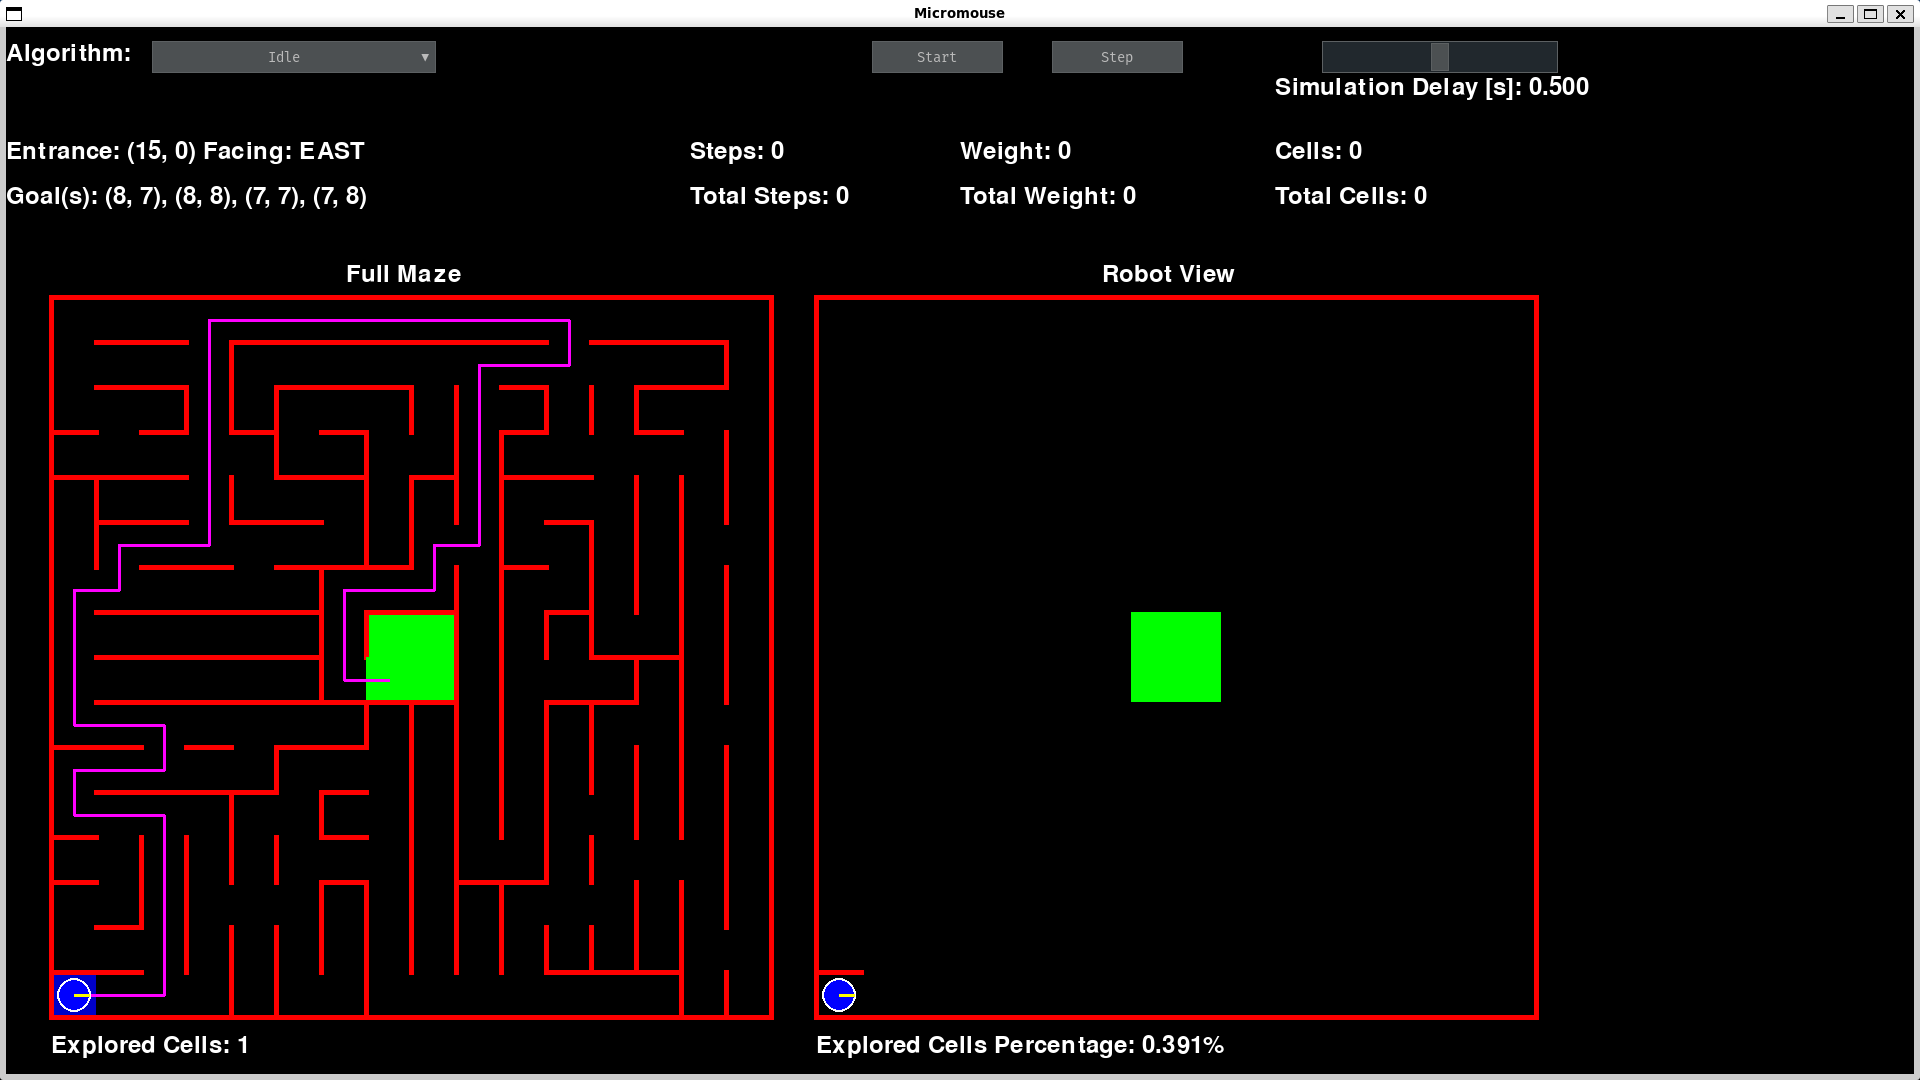
\includegraphics[width=\textwidth]{images/simulation_start.png}
\caption{Simulation screen}
\label{Simulation screen}
\end{figure}

The simulation's controls in figure \ref{Simulation controls close-up} include various components:
\begin{itemize}
    \item Drop-down menu to choose which algorithm to use to try and solve the \gls{maze}. Initially set to \textit{idle}.
    \item A start/stop button to make the robot start executing the algorithm or stop it mid-run and then start again from the same spot.
    Initially set to \textit{stop} as the simulation starts executing the algorithm as soon as it is chosen.
    \item A step button to make the robot perform a single move operation.
    \item A simulation delay slider to control how much time is added to each step.
    \item Information about the \gls{maze} such as the coordinates of the starting and goal \gls{cell}s and the direction the robot is facing at the start of the simulation. This information is loaded with the \gls{maze} and cannot be modified directly.
    \item Information about the robot's path is displayed by three counters.
    The \textit{step} counter shows the number of actions the robot has done in the current run and the total amount.
    The \textit{weight} counter shows the weight of the path from the starting \gls{cell} of the current run and the total weight.
    The \textit{cell} counter shows the number of \gls{cell}s the robot has gone through in the current run and the total amount.
    Note that this counter does not count unique \gls{cell}s. 
\end{itemize}

\begin{figure}[H]
\centering
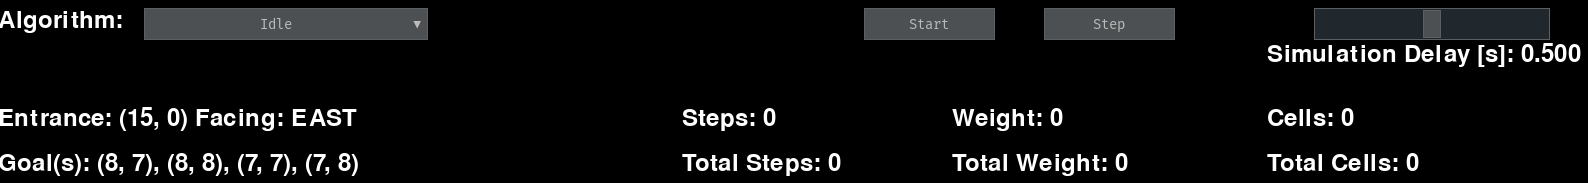
\includegraphics[width=\textwidth]{images/simulation_HUD.png}
\caption{Simulation controls close-up}
\label{Simulation controls close-up}
\end{figure}

Moreover, the simulation displays two more statistics at the bottom of the screen: the number of explored \gls{cell}s and their percentage.

\begin{figure}[H]
\centering
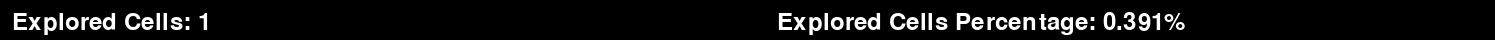
\includegraphics[width=\textwidth]{images/simulation_HUD_bot.png}
\caption{Simulation bottom close-up}
\label{Simulation bottom close-up}
\end{figure}

\subsubsection{Heat Map}
\paragraph{}
As the simulation executes the robot's algorithm a heat map is generated on the full \gls{maze} view.
Each \gls{cell} is colored from cool to warm to indicate how many actions the robot has performed in each \gls{cell}.
All \gls{cell}s start without a color.
After every action, the color of the \gls{cell} at the robot's position gets warmer.
The color of the \gls{cell} can be one of the following: blue, cyan, green, yellow, orange, red, and brown.
Blue means the robot has performed one action in that \gls{cell} while brown means the robot has performed at least seven actions in that \gls{cell}.
A 90\textdegree\ turn is composed of 2 actions: rotating the robot and moving forward.
As such, a 90\textdegree\ turn counts as 2 steps, and a 180\textdegree\ counts as 3 steps.
An example of a heat map can be seen in figure \ref{Heat map example} where a right wall follower robot is attempting to solve the \gls{maze}.

\begin{figure}[H]
\centering
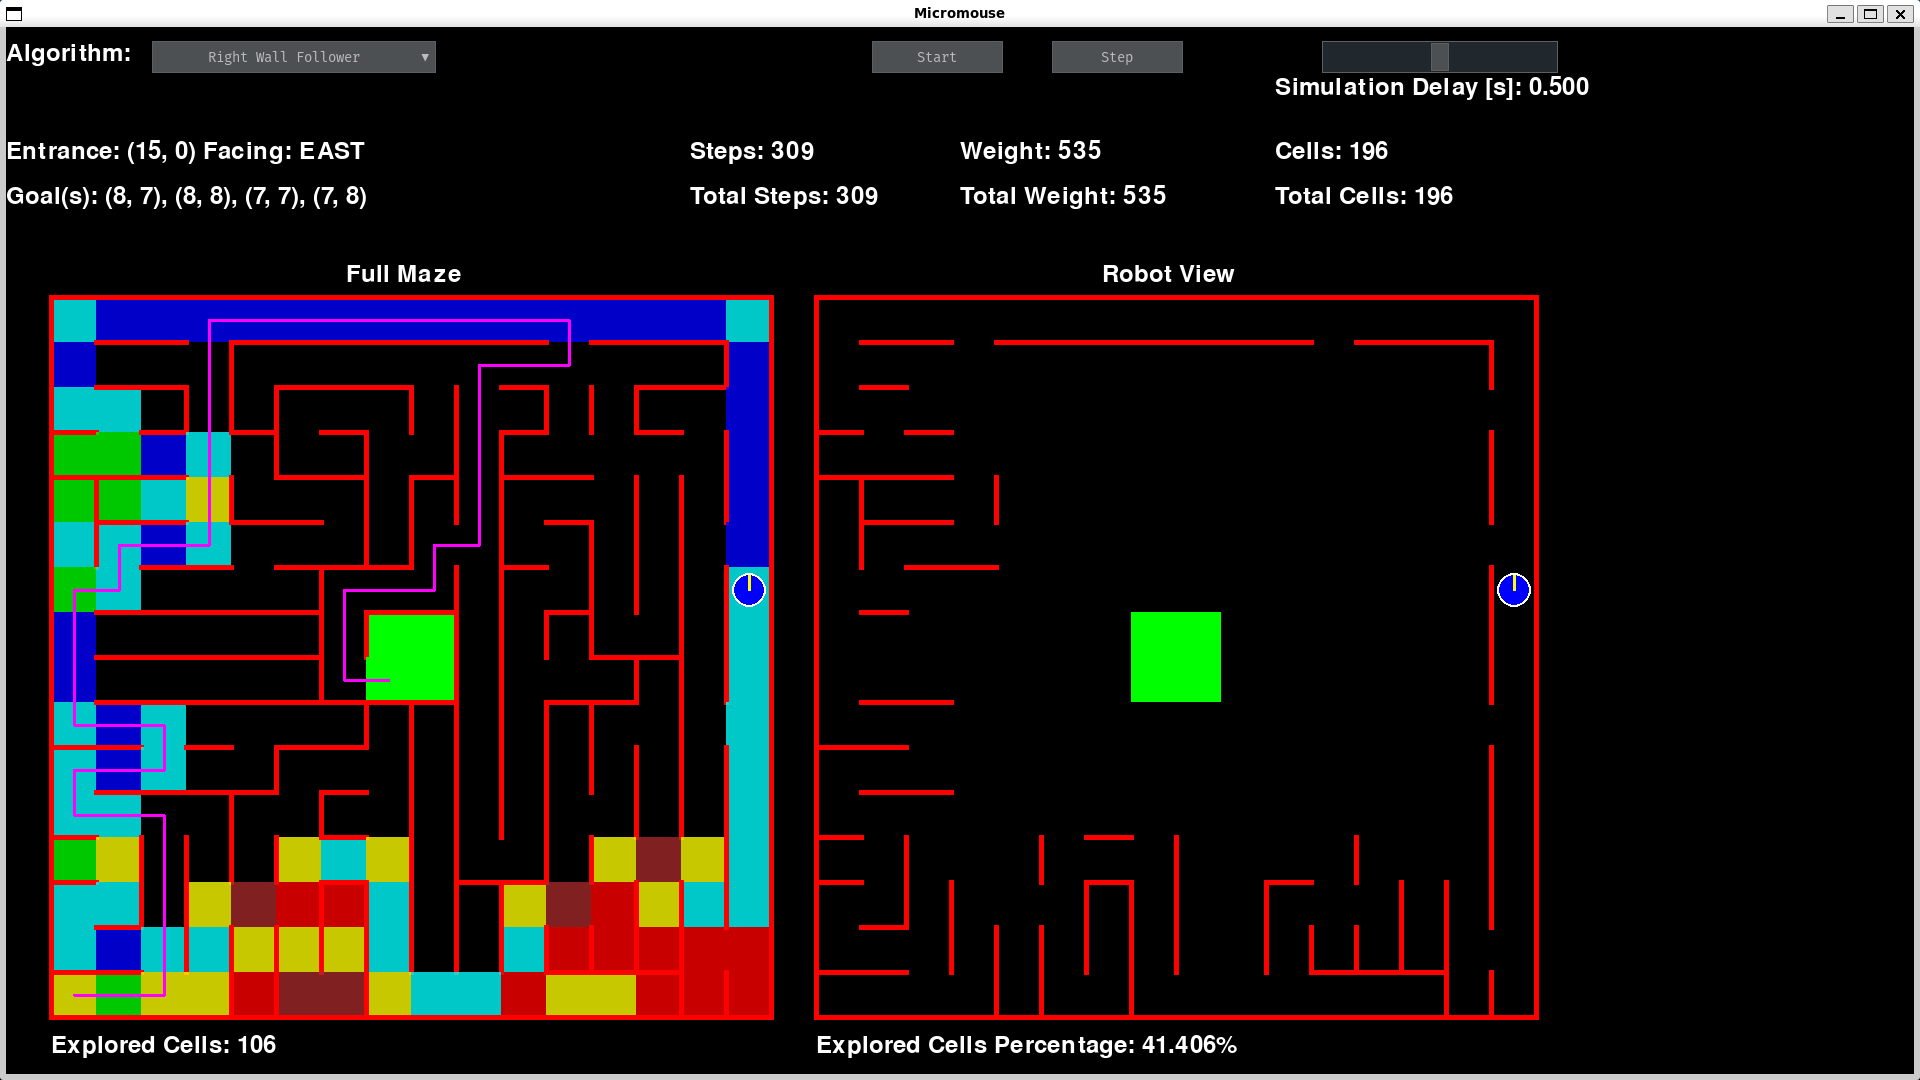
\includegraphics[width=\textwidth]{images/simulation_heatmap.png}
\caption{Heat map example}
\label{Heat map example}
\end{figure}

The heat map scale index is provided in figure \ref{Heat map scale}.

\begin{figure}[H]
\centering

\includegraphics[width=\textwidth]{images/heatmap.png}
\caption{Heat map scale index}
\label{Heat map scale}
\end{figure}

\subsubsection{Additional Cell Information}
\paragraph{}
The simulation provides an easy way for an algorithm to save additional information about the \gls{maze}.
In addition, this information will be displayed by the simulation on the \gls{maze}.
The additional information that can be added to each \gls{cell} is:
\begin{enumerate}
    \item Weight - A numeric value the algorithm can assign to the \gls{cell}, meant to be used by algorithms that use weights.
    \item Color - The color of the \gls{cell}.
    Can be used to add visualization to the algorithm. 
    \item Visited - A counter that can be used to keep track of how many times the robot has visited a \gls{cell}. This value is automatically incremented by the simulation after every robot action.
\end{enumerate}

\subsubsection{Special Flood-Fill Information}
\paragraph{}
The flood-fill algorithm, which is explained in section \ref{Flood-Fill Algorithm}, stores the distances of each \gls{cell} from the goal.
When simulating an algorithm that uses the flood-fill algorithm to explore the \gls{maze}, the currently stored distances of each \gls{cell} from the goal are displayed in the robot's view.
In addition, the robot's path is traced as it moves across the \gls{maze}.
An example of the additional information provided for flood-fill-based algorithms can be seen in figure \ref{Extra information for flood-fill-based algorithms} where a flood-fill robot is attempting to solve the \gls{maze}.

\begin{figure}[H]
\centering
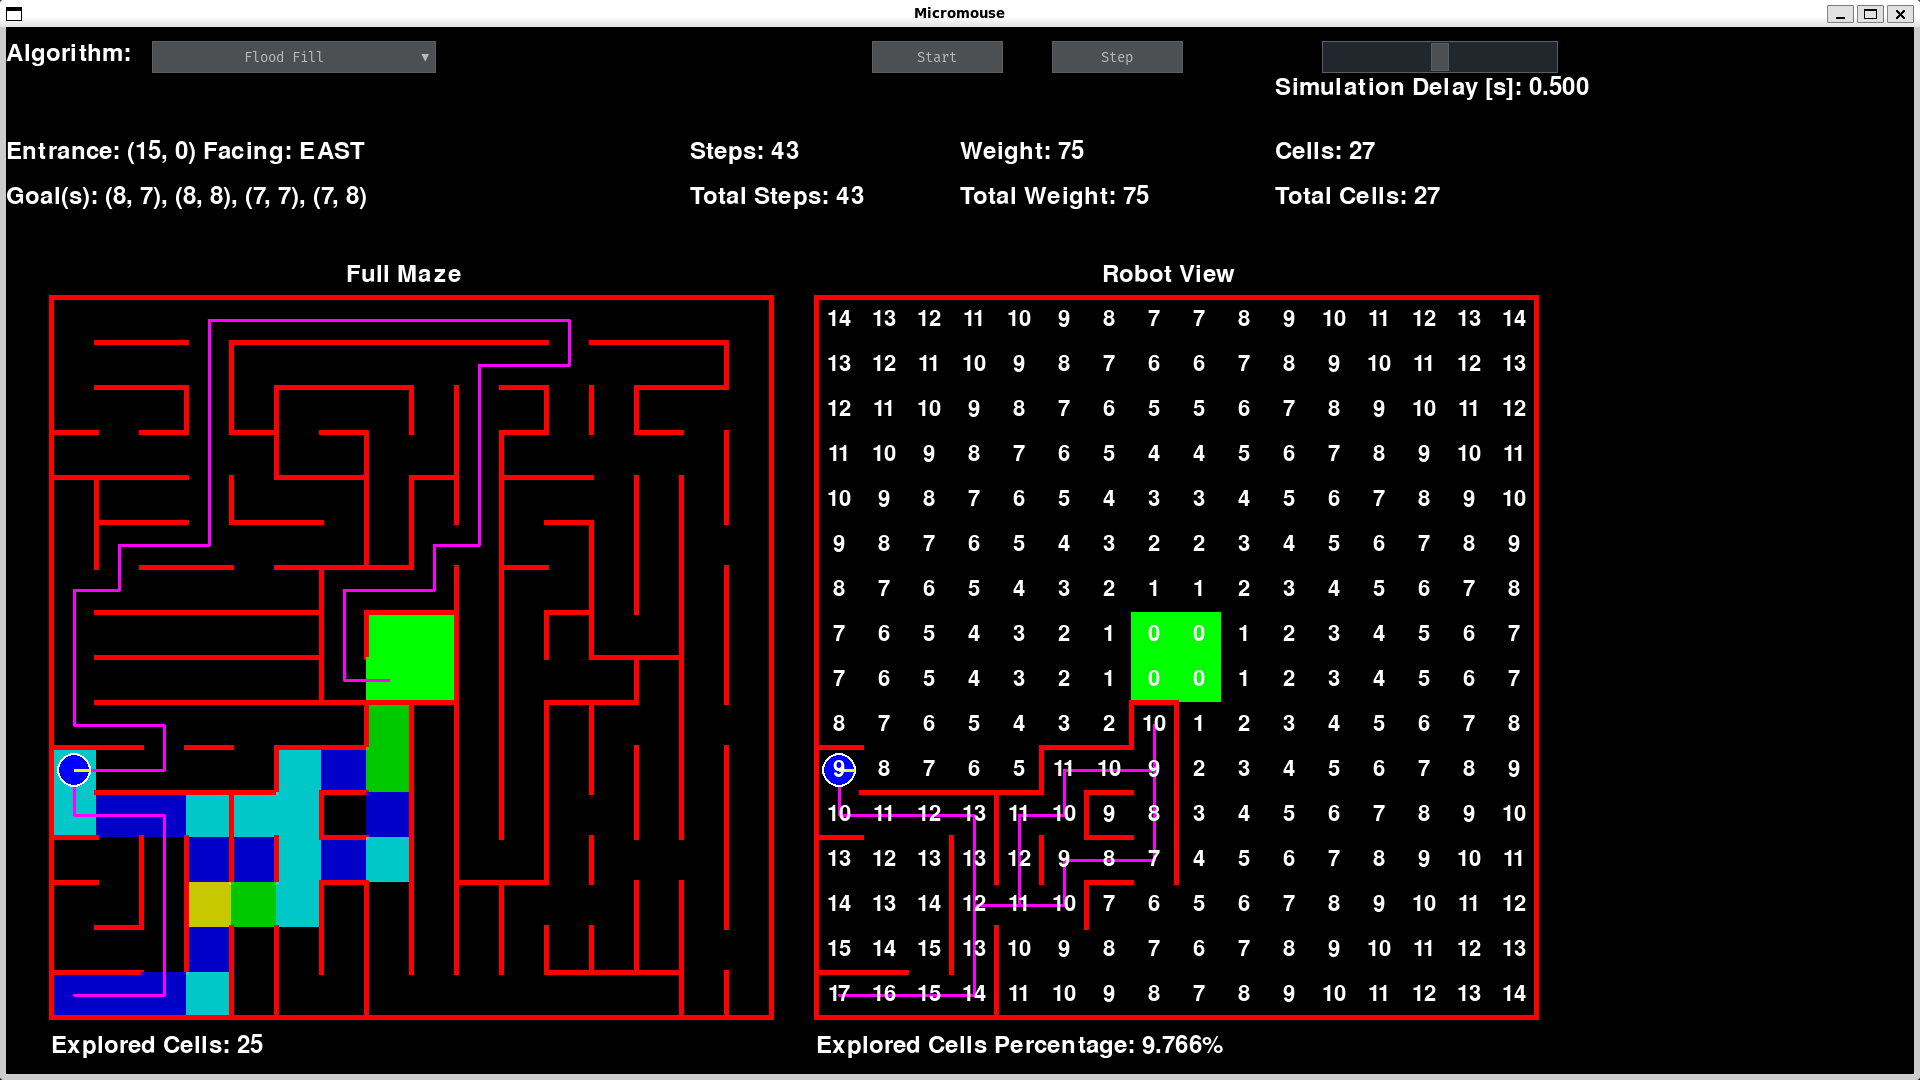
\includegraphics[width=\textwidth]{images/simulation_flood_fill.png}
\caption{Extra information for flood-fill-based algorithms}
\label{Extra information for flood-fill-based algorithms}
\end{figure}

\subsubsection{Special Dijkstra's Algorithm Information}
\paragraph{}
The Dijkstra's algorithm, which is explained in section \ref{Dijkstra's Algorithm}, calculates the minimum distances of each \gls{cell} from the starting \gls{cell}.
When simulating an algorithm that uses Dijkstra's algorithm to solve the \gls{maze}, the calculated distances of each \gls{cell} from the starting \gls{cell} are displayed in the robot's view.
In addition, the robot's path is traced as it moves across the \gls{maze}.
An example of the additional information provided for Dijkstra-based algorithms can be seen in figure \ref{Simulating flood-fill combined with Dijkstra's algorithm} where each \gls{cell} contains the distance from the starting \gls{cell} calculated by Dijkstra's algorithm with the defined time weights for each action.
In addition, a \gls{cell} that was not explored or is not reachable, is colored accordingly.

\subsubsection{Other Algorithm's Information}
\paragraph{}
Specific algorithms can color the \gls{maze}'s \gls{cell} to display information about the execution of the algorithm.
For example, our new proposed algorithm, Thorough Flood-Fill explained in section \ref{thorough flood-fill algorithm}, uses different colors for \gls{cell}s based on its current state:
\begin{itemize}
    \item \Gls{cell}s that are unexplored, can be seen in figure \ref{thorough flood-fill exploring}.
    \item The \gls{cell} that is the current exploration goal, can be seen in figure \ref{thorough flood-fill exploring}.
    \item \Gls{cell}s that are considered as a dead-end, can be seen in figures \ref{Before dead-end detection}, \ref{After dead-end detection}, \ref{Before dead-end detection using flood-fill}, and \ref{After dead-end detection using flood-fill}.
\end{itemize}

\subsection{Generic Algorithm Test Environment}
\paragraph{}
The code is structured to ease the process of adding and testing new algorithms.
The intent is to provide a platform for testing \gls{Micromouse} algorithms easily.
Moreover, the GUI is replaceable if you want to render the simulation differently or present different information about the algorithm.
The technical details of adding new algorithms or changing the GUI are explained in detail in the code repository.
A link to the code repository can be found in section \ref{Project Repo}.

\section{Na\"{i}ve Algorithms} \label{naive-algorithms}
\paragraph{}
The algorithms in this section have been implemented for the initial testing of the simulation environment. The main usage of those algorithms is to check the integration between the different components, mainly, the \gls{maze} representation and the simulation environment. They are not intended to solve the \gls{Micromouse} challenge. In addition, for simpler \gls{maze}s, which those algorithms can solve in a reasonable time, they can be used as a starting point for improvement.

\subsection{Random Path Algorithm} \label{Random Algorithm}
\paragraph{}
In this approach, the robot sees which walls surround it for each step and randomly decides where to go.
This simple logic can be demonstrated by the following algorithm:
\begin{enumerate}
    \item Randomly choose a \gls{cell} which is one step away and has no wall blocking it and move to it.
    \item If current \gls{cell} is not the goal, go back to step 1, else finish.
\end{enumerate}
This approach does not provide a robust solution to the problem.
Most of the time, the robot will not find the goal in a reasonable time and therefore, will not be able to successfully solve the \gls{Micromouse} challenge.

\subsection{Wall-Following Algorithm} \label{Wall Following Algorithm}
\paragraph{}
The wall-following algorithm is divided into two:
\begin{enumerate}
    \item Left wall-following algorithm
    \item Right wall-following algorithm
\end{enumerate}
Both algorithms are almost identical with the only difference being which wall to follow.
For instance, the logic for a right wall follower robot can be demonstrated by the following algorithm:
\begin{enumerate}
    \item If current \gls{cell} has no wall to the right of the robot then turn right.
    \item If current \gls{cell} has no wall in front of the robot then move forward, else turn left.
    \item If current \gls{cell} is the goal, stop, else return to step 1.
\end{enumerate}
The algorithm for a left wall follower robot is achieved by replacing all instances of the word 'right' with the word 'left' and all instances of the word 'left' with the word 'right' in the algorithm presented above.
As discussed in section \ref{introduction}, the wall-following algorithm is not suitable for solving the \gls{Micromouse} challenge. A robot utilizing this algorithm will most likely never reach the goal because the \gls{maze} is deliberately constructed in a way that prevents using wall-following techniques.

\section{Sophisticated Algorithms} \label{sophisticated-algorithms}
\subsection{Dijkstra's Algorithm} \label{Dijkstra's Algorithm}
\subsubsection{Description}
\paragraph{}
An algorithm for finding the shortest paths between nodes in a directed weighted \gls{graph}.
The algorithm can be described in pseudo-code as follows:

\begin{lstlisting}[mathescape, caption={Dijkstra's algorithm pseudo-code}, captionpos=b]
Dijkstra(graph, source):
    distance $\leftarrow$ empty array
    previous $\leftarrow$ empty array
    Q $\leftarrow$ empty queue
    for each vertex v in graph:
        distance[v] $\leftarrow$ $\infty$
        previous[v] $\leftarrow$ NULL
        add v to Q
    distance[source] $\leftarrow$ 0
    while Q is not empty:
        u $\leftarrow$ vertex in Q with minimum distance
        remove u from Q
        for each edge e in graph connecting u and v:
            new_distance $\leftarrow$ distance[u] + weight of e
            if new_distance < distance[v]:
                distance[v] $\leftarrow$ new_distance
                previous[v] $\leftarrow$ u
    return distance, previous
\end{lstlisting}

The \textit{distance} array is the current distance from the source to each vertex.
The \textit{previous} array contains pointers to the previous-hop nodes on the shortest path from the source to the given vertex.
Given a directed weighted \gls{graph} and a source node, we can calculate the distance and the shortest route to every other node in the \gls{graph} from the source node.

Therefore, representing the \gls{maze} as a directed weighted \gls{graph} with the start \gls{cell} as the source node and applying Dijkstra's algorithm, will allow finding the shortest or fastest route in the \gls{maze}.

\subsubsection{Maze as a Directed Weighted Graph} \label{Maze as a Directed Weighted Graph}
\paragraph{}
To use Dijkstra's Algorithm, first, the \gls{maze} must be represented as a directed weighted \gls{graph}.
Each \gls{cell} in the \gls{maze} is represented by up to four vertices in the \gls{graph}.
Those vertices correspond to the direction the robot is facing while located at that \gls{cell} - North, East, South, and West.
Each vertex appears if the corresponding wall does not exist.
Because the robot rotation is limited to 90\textdegree\ left or right, there is an edge connecting the north vertex to the east and west vertices.
Because the robot can move forward, there is an edge connecting the north and south vertices.
The same applies to the east, south, and west vertices.
Therefore, it can be viewed as a \gls{graph} connecting the missing walls of the \gls{cell}s.
The representation of a single \gls{cell} as a directed \gls{graph} is demonstrated in the following figure.

\begin{figure}[H]
\centering
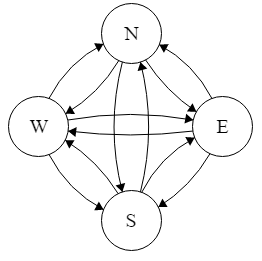
\includegraphics[width=0.4\textwidth]{images/cell_graph.png}
\caption{A \gls{cell} as a directed \gls{graph}}
\end{figure}

The weight of each edge can be changed to achieve different definitions of the fastest route.
For example, setting the weight of all edges to 1 will result in finding the shortest path with the least amount of moving forward and turning.

Since we care about the fastest route rather than the shortest one, our implementation uses time units for weights. An arbitrary unit of 1 was decided for moving the distance of a single cell forward. Acceleration and deceleration were both also given a weight of 1 and a 90\textdegree\ turn was given a base weight of 2. A turn is composed of a decelerate-turn-accelerate sequence and therefore gets a total weight of $1 + 2 + 1 = 4$ in the graph to accommodate the necessary velocity changes.
% There's also a special vertex for the starting point that we may want to mention...
% Maybe we can include that special one, but I'm not sure...

To allow movement between the different \gls{cell}s, two zero-weight edges connect each shared wall vertices.
An example of 4 adjacent \gls{cell}s with no walls as a directed weighted \gls{graph} is shown in figure \ref{No walls maze as a directed weighted graph figure}. The coordinates of each \gls{cell} are written alongside the direction of the wall.

\begin{figure}[H]
\centering
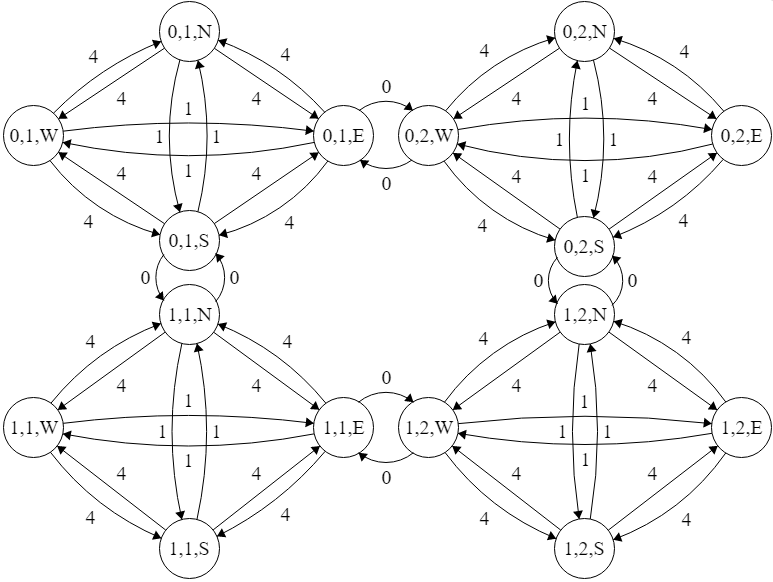
\includegraphics[width=0.78\textwidth]{images/four_cell_graph_with_weights.png}
\caption{Four \gls{cell}s with no walls as a directed weighted \gls{graph}}
\label{No walls maze as a directed weighted graph figure}
\end{figure}

Next, the representation of the following sample \gls{maze} as a directed weighted graph is shown in figure \ref{Sample maze as a directed weighted graph figure}.
\lstset{
  xleftmargin=\simpleMazeMargin,
  xrightmargin=\simpleMazeMargin
}
\begin{lstlisting}
    +---+---+---+
    |       |   |
    +   +   +   +
    |   |       |
    +---+---+---+
\end{lstlisting}

\begin{figure}[H]
\centering
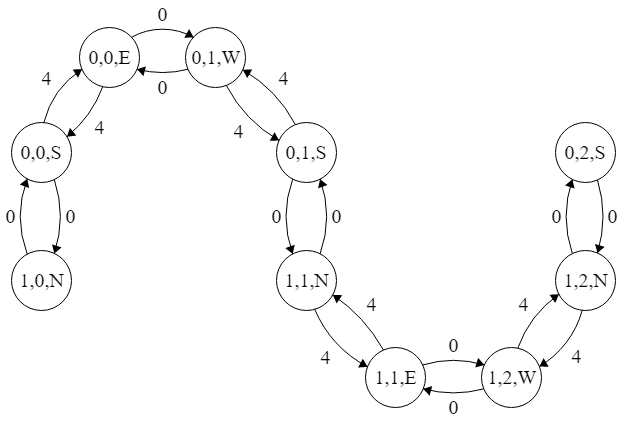
\includegraphics[width=\textwidth]{images/sample_maze_graph.png}
\caption{Sample maze as a directed weighted \gls{graph}}
\label{Sample maze as a directed weighted graph figure}
\end{figure}

The coordinates of each \gls{cell} are written alongside the direction of the wall.
Note that each \gls{cell} in figure \ref{Sample maze as a directed weighted graph figure} only has nodes where the \gls{cell} has no walls. This can save a lot of memory and computation time for algorithms that use the resulting \gls{graph}.

\subsubsection{Complexity} \label{Dijkstra's Algorithm Complexity}
\paragraph{}
The time complexity for Dijkstra's algorithm is given by $O(|V| + |E|\log |V|)$ where $|V|$ is the number of vertices in the \gls{graph} and $|E|$ is the number of edges in the \gls{graph}.
The \gls{auxiliary space} complexity of the algorithm is $O(|V|)$ where $|V|$ is the number of vertices in the \gls{graph}.
The number of vertices in the \gls{graph}, $|V|$, is proportional to the number of \gls{cell}s in the \gls{maze}.
Likewise, the number of edges in the \gls{graph}, $|E|$, is proportional to the number of vertices in the \gls{graph}.
Therefore, the time complexity for this algorithm can be written as $O(n\log n)$ where $n$ is the number of \gls{cell}s in the \gls{maze}. 
In addition, the \gls{auxiliary space} complexity of the algorithm can be written as $O(n)$ where $n$ is the number of \gls{cell}s in the \gls{maze}.

\subsubsection{Drawbacks} \label{Dijkstra's algorithm drawbacks}
\paragraph{}
As discussed in section \ref{introduction}, the robot has no prior knowledge about the \gls{maze}.
This limitation and the fact that Dijkstra's algorithm is not a \gls{graph} traversing algorithm, mean the \gls{maze} must be explored by other means before using Dijkstra's algorithm. 

\subsection{Flood-Fill Algorithm} \label{Flood-Fill Algorithm}
\subsubsection{Description}
\paragraph{}
Unlike Dijkstra's algorithm, discussed in section \ref{Dijkstra's Algorithm}, this algorithm assumes no prior knowledge about the \gls{maze}.
This property and its simplicity make it an extremely popular algorithm used in the \gls{Micromouse} competition.
The robot takes the most optimistic path to the goal.
In each step the robot follows the next logic:
\begin{enumerate}
    \item Update the \gls{maze} to include the current \gls{cell}'s walls.
    \item Update the distances from every \gls{cell} in the \gls{maze} to the goal based on the currently known walls in the \gls{maze}.
    \item Move to the \gls{cell} with the lowest distances from the goal among the \gls{cell}s adjacent to the current \gls{cell}. If more than one applies choose one at random.
\end{enumerate}

The process resembles flooding the \gls{maze} with water and updating values based on the flow.
This resemblance gives the algorithm its name.
Once the robot reaches the goal it can optimize the path it took by looking back and choosing the path following the trail of decreasing distances from the goal.

\subsubsection{Complexity}
\paragraph{}
The time complexity for this algorithm is given by $O(n)$ where $n$ is the number of \gls{cell}s in the \gls{maze}.
The \gls{auxiliary space} complexity of the algorithm is $O(n)$ where $n$ is the number of \gls{cell}s in the \gls{maze}.
As can be seen, the complexity of this algorithm is better than the complexity of Dijkstra's algorithm, described in section \ref{Dijkstra's Algorithm Complexity}, giving it a shorter execution time.

\subsubsection{Finding the Shortest Path} \label{Flood Fill - Finding the Shortest Path}
\paragraph{}
In a \gls{Micromouse} competition the robot needs to get back to the starting \gls{cell} on its own to start the next run or a time penalty is issued, as noted in section \ref{Competition Rules}.
The flood-fill algorithm takes advantage of the return trip to further optimize the path.
Once the robot reaches the goal, the return trip is a backward flood-fill, meaning the goal is the new starting \gls{cell} and the starting \gls{cell} is the new goal.
Adding a bias to the flood-fill algorithm which tries to avoid \gls{cell}s already visited by the robot on the way to the goal, makes the return trip different.
The bias is added by giving more weight to \gls{cell}s the robot has already visited.

For example, the robot can store one bit for each \gls{cell} in the \gls{maze}.
This bit will be denoted as the \textit{visited bit}.
The \textit{visited bit} will store whether the robot has already visited the \gls{cell}.
On the way back from the goal, the weight of each \gls{cell} will be the distance from the starting \gls{cell} plus the value of the \textit{visited bit}.
This will increase the weight of \gls{cell}s already visited by 1 and will make the robot less likely to travel through those \gls{cell}s on the way back.

Once the robot reaches the start it can optimize the path it took by looking back and choosing the path following the trail of decreasing distances.
Between these two attempts, one of them is likely to be the shortest path in the sense of the least amount of \gls{cell}s required to reach the goal.

\subsubsection{Drawbacks} \label{Flood-fill drawbacks}
\paragraph{}
The flood-fill algorithm is simple and fast and does not assume any prior knowledge about the \gls{maze}.
This makes it a very fitting algorithm for solving the \gls{Micromouse} challenge.
However, the result of this algorithm is the shortest path from the starting \gls{cell} to the goal, which is not guaranteed to be the fastest route the robot can take.
The winner of the \gls{Micromouse} competition is the robot that reached the goal in the least amount of time, as noted in section \ref{scoring}.
The shortest path to the goal could have a lot of turns which will slow down the robot, while another longer path utilizes more straight lines the robot can race through much faster.
Therefore, finding the shortest path is not always the best solution to the problem.
A way to add weights that represent the time it takes for each action to complete is needed.
Unfortunately, the flood-fill algorithm alone is not suitable for this kind of task.

\section{The New Proposed Algorithm - Thorough Flood-Fill} \label{new-algorithm}
\subsection{Prologue}
\paragraph{}
Up to this point, a way to solve a known \gls{maze} while finding the fastest path was discussed in section \ref{Dijkstra's Algorithm}.
Moreover, a way to solve an unknown \gls{maze} while also finding the shortest path was discussed in section \ref{Flood-Fill Algorithm}.
The new proposed algorithm utilizes the flood-fill algorithm to explore the \gls{maze} and Dijkstra's algorithm to find the fastest path by the given time weights.

\subsection{Combining the Flood-Fill Algorithm with Dijkstra's Algorithm} \label{Combining Flood-Fill with Dijkstra's Algorithm}
\subsubsection{Description}
\paragraph{}
At the start, the robot has no knowledge about the walls of the \gls{maze} except for the walls of the starting \gls{cell}.
The flood-fill algorithm is used to get from the starting \gls{cell} to the goal.
Once the robot has reached the goal, it uses the flood-fill algorithm to navigate back from the goal to the starting \gls{cell} in a different path, as described in section \ref{Flood Fill - Finding the Shortest Path}.
Now, the robot has acquired some knowledge about the \gls{maze} and found at least two different routes leading from the starting \gls{cell} to the goal.
For the solution, instead of following the shortest path between the two attempts, the robot finds the fastest one according to Dijkstra's algorithm is chosen, even if it is longer.

Even though not all the \gls{maze} has been explored, the algorithm presented in section \ref{Maze as a Directed Weighted Graph} is still viable.
To use that algorithm, unexplored \gls{cell}s are treated as having four walls.
Therefore, unexplored \gls{cell}s are excluded from the \gls{graph} and ignored by Dijkstra's algorithm.
As seen in figure \ref{Simulating flood-fill combined with Dijkstra's algorithm}, unexplored \gls{cell}s are assigned a weight of $inf$ to indicate that the robot can't reach them.

\begin{figure}[H]
\centering
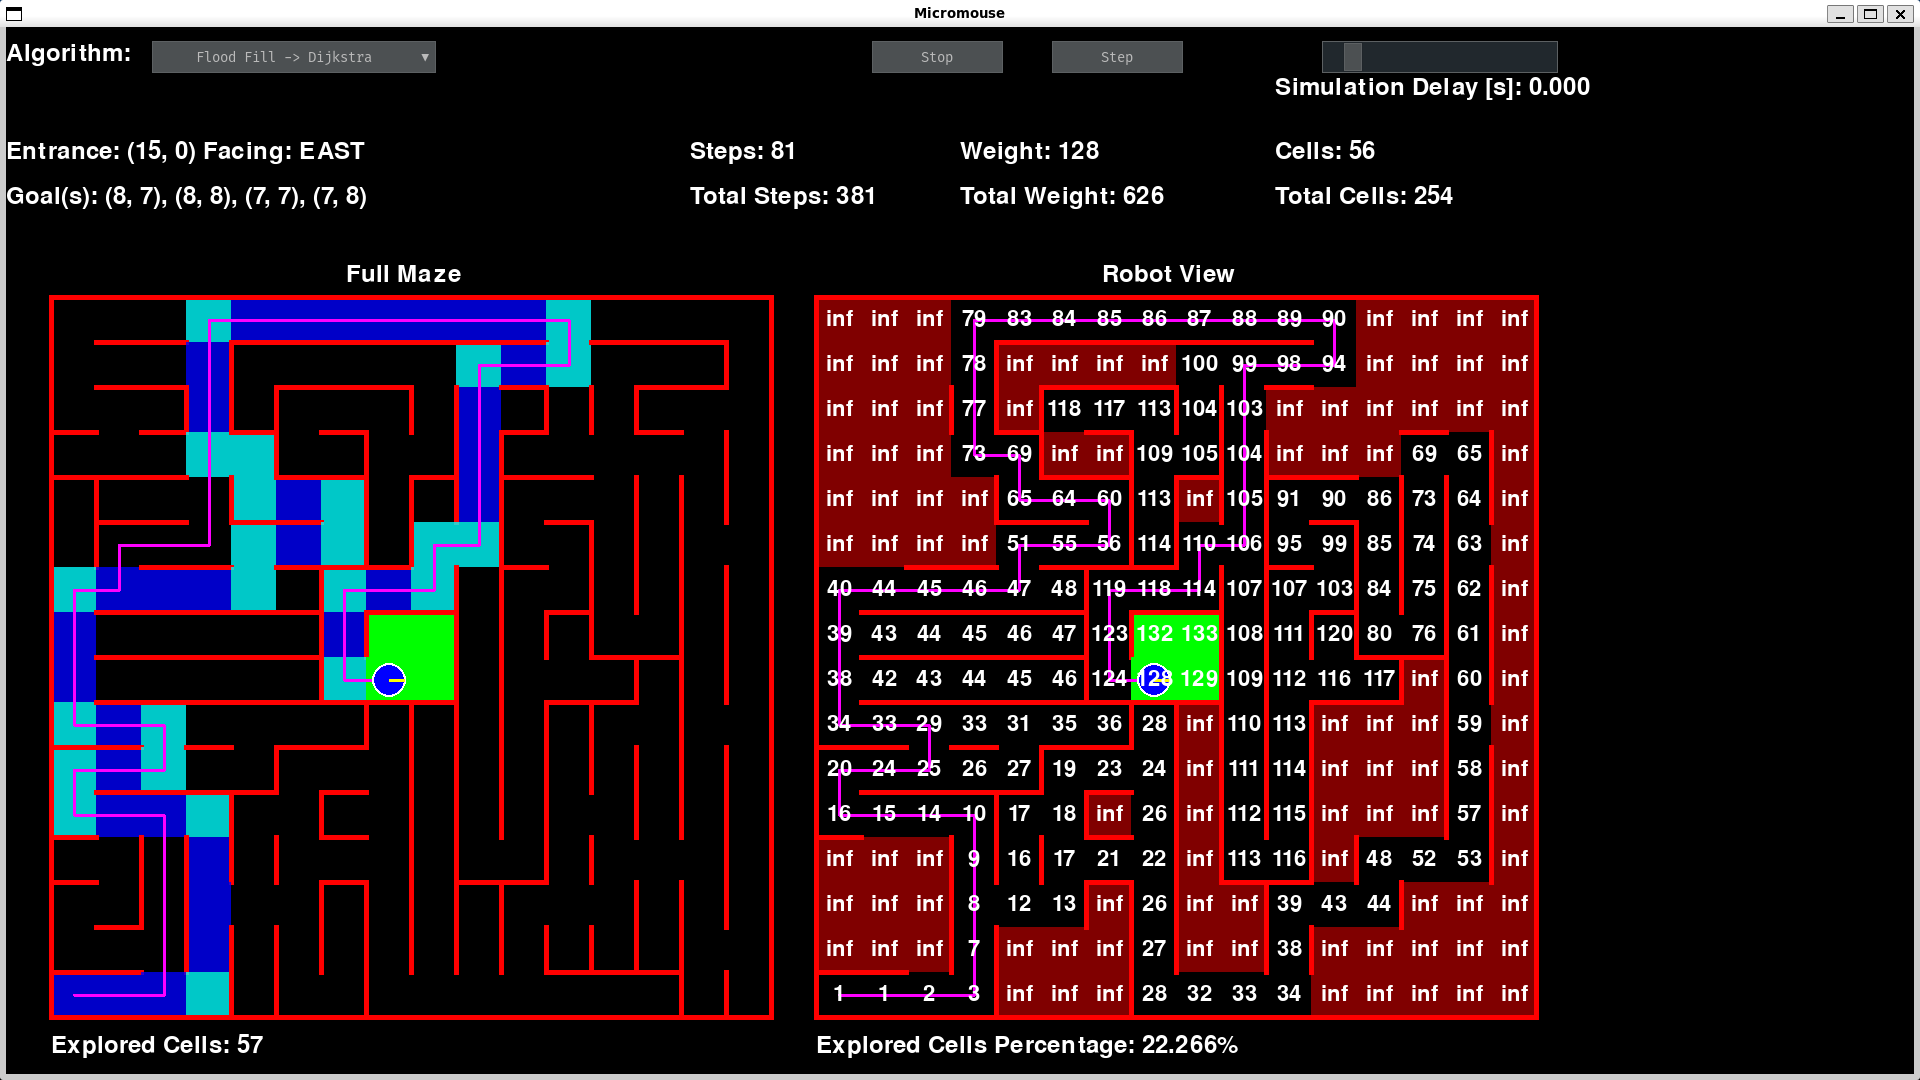
\includegraphics[width=\textwidth]{images/floodijkstra.png}
\caption{Simulating flood-fill combined with Dijkstra's algorithm}
\label{Simulating flood-fill combined with Dijkstra's algorithm}
\end{figure}

By combining the two algorithms the robot can explore an unknown \gls{maze} and find the fastest route.
This approach allows leveraging each algorithm's advantage while alleviating its disadvantages.

\subsubsection{Drawbacks}
\paragraph{}
As discussed in section \ref{Flood-Fill Algorithm}, the flood-fill algorithm does not explore all the \gls{maze}.
Therefore, although it gives a good solution to the \gls{maze}, which can be the optimal solution according to the defined time weights of each action, it is not guaranteed to be optimal.

\subsection{Thorough Flood-Fill Algorithm} \label{thorough flood-fill algorithm}
\subsubsection{Description}
\paragraph{}
The \textit{Thorough Flood-Fill} algorithm is our new proposed solution.
The name is based on the intensive exploration of the \gls{maze} using the flood-fill algorithm.
We want to use the algorithm discussed in section \ref{Combining Flood-Fill with Dijkstra's Algorithm} while guaranteeing it can find the optimal solution.
To achieve this, we should explore more regions of the \gls{maze}.
The downside of exploring more areas of the \gls{maze} is that it takes time off of the allocated time of access to the \gls{maze}, as noted in section \ref{Competition Rules}.
Therefore, the algorithm will prioritize finding the goal and then use the remaining time to explore the \gls{maze} as much as possible before returning to the starting \gls{cell} and finding the fastest route.

\subsubsection{Mapping Unexplored Regions}
\paragraph{}
After finding a path from the starting \gls{cell} to the goal, the robot explores the \gls{maze} as much as possible.
To achieve that, once the robot reaches the goal, it performs the following exploration logic:
\begin{enumerate}
    \item Sort all unexplored \gls{cell}s in the \gls{maze} into groups of connected unexplored \gls{cell}s.
    The robot has no knowledge about the walls surrounding those \gls{cell} yet. Therefore, unexplored \gls{cell}s are in the same group if there could be a path between them that does not cross an already explored \gls{cell}.
    \item Perform a flood-fill algorithm from the current \gls{cell} to the \gls{cell} that is furthest away from the current \gls{cell} and is part of the largest group of unexplored \gls{cell}s.
    This \gls{cell} is the next goal.
    \item When reaching the next goal, mark it as the starting \gls{cell} and return to step 1.
\end{enumerate}

The simulation supports visual aids for the exploration part of the algorithm.
As the robot reaches the goal, it turns to explore other areas of the \gls{maze}.
An example of mapping the \gls{maze} can be found in figure \ref{thorough flood-fill exploring}.
Unexplored \gls{cell}s are marked with a different color on the robot's view of the \gls{maze} (right).
The robot has marked the $(0,0)$ \gls{cell} as its current destination and is heading there.

\begin{figure}[H]
\centering
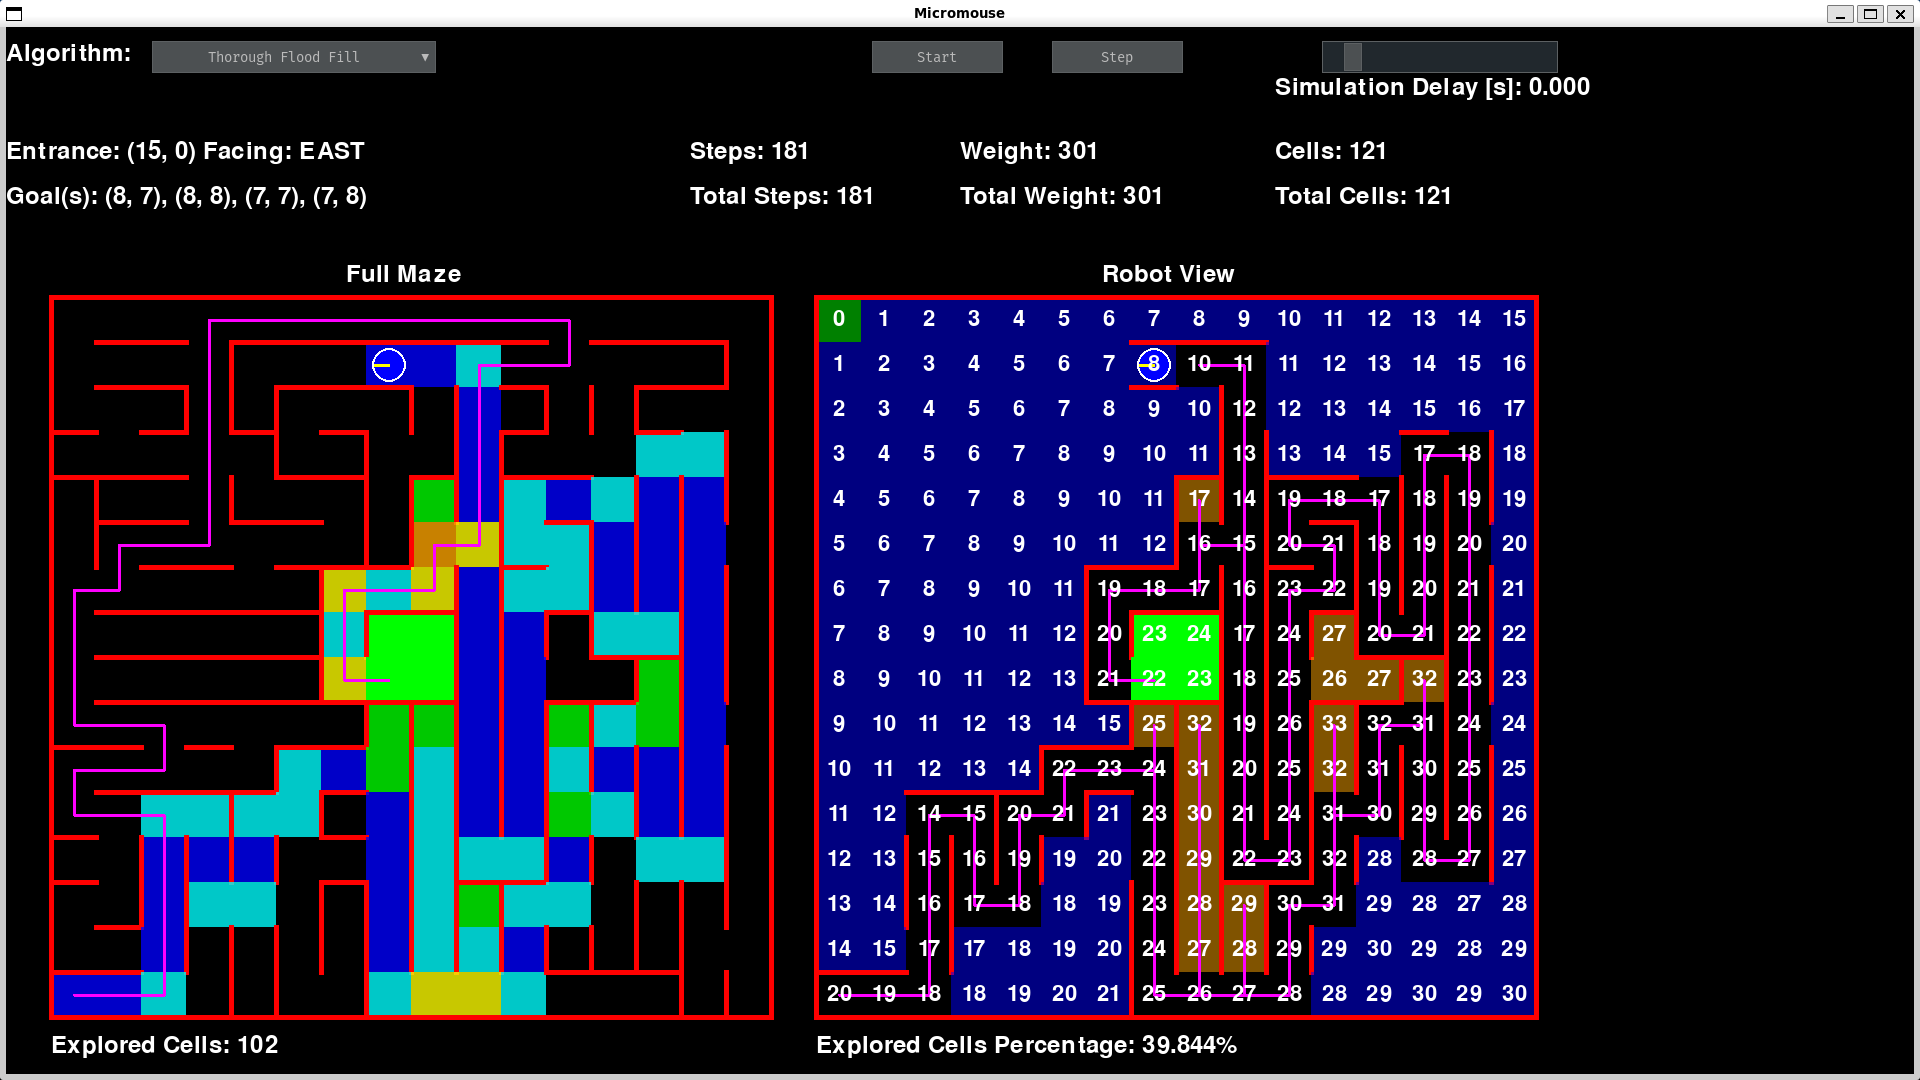
\includegraphics[width=\textwidth]{images/thorough_search.png}
\caption{Robot exploring the \gls{maze} using the thorough flood-fill algorithm}
\label{thorough flood-fill exploring}
\end{figure}

The exploration logic continues until the robot has explored enough \gls{cell}s in the \gls{maze}.
While exploring the \gls{maze}, the robot needs to avoid the starting \gls{cell} because this will start a new run, as noted in section \ref{Competition Rules}.
Stepping in the starting \gls{cell} can end the exploration run prematurely.
An infinite weight is assigned to the starting \gls{cell} so that no route will go through it to avoid this problem.
When the explored \gls{cell}s percentage in the \gls{maze} is higher than the threshold, the robot stops exploring the \gls{maze}.
Next, the robot sets the starting \gls{cell} as its next goal and uses Dijkstra's algorithm to find the fastest route from its current \gls{cell} to the starting \gls{cell}.
The fast run will start once the robot reaches the starting \gls{cell}.
The robot uses Dijkstra's algorithm to find the fastest route from the starting \gls{cell} to the goal.

\subsubsection{Dead-End Detection}
\paragraph{Rationale}
Given a directed weighted \gls{graph} for a \gls{maze}, Dijkstra's algorithm can find the fastest path.
As explained in section \ref{Dijkstra's algorithm drawbacks}, Dijkstra's algorithm needs a large amount of information about the \gls{maze} to find the optimal path.
Therefore, we want the robot to explore the minimum number of \gls{cell}s that still allows Dijkstra's algorithm to find the optimal path.

\paragraph{Adding Imaginary Walls}
To reduce the exploration time, once the robot has enough information about a group of \gls{cell}s, it can deduce that the group is considered a dead-end and not explore that group further.
While the robot explores the \gls{maze}, it tries to add walls around itself.
If the wall's addition does not break the \gls{maze}'s connectivity (the goal \gls{cell}s, the starting \gls{cell}, and the robot's current \gls{cell} are all still connected) and creates a \gls{cell} group that is separate from the rest of the \gls{maze}, this \gls{cell} group is considered a dead-end.
The group is then colored with a distinct color to stand out.

Figure \ref{Before dead-end detection} demonstrates \gls{cell}s marked as a dead-end.
Notice the three \gls{cell} group to the robot's right, which is not marked as a dead-end.
The region of interest is marked on the image with a circle.
Those \gls{cell}s are not leading anywhere.
By adding an imaginary eastern wall in the current \gls{cell}, this group is disconnected from the \gls{maze} and does not contain the starting \gls{cell}, the goal, or the robot.

\begin{figure}[H]
\centering
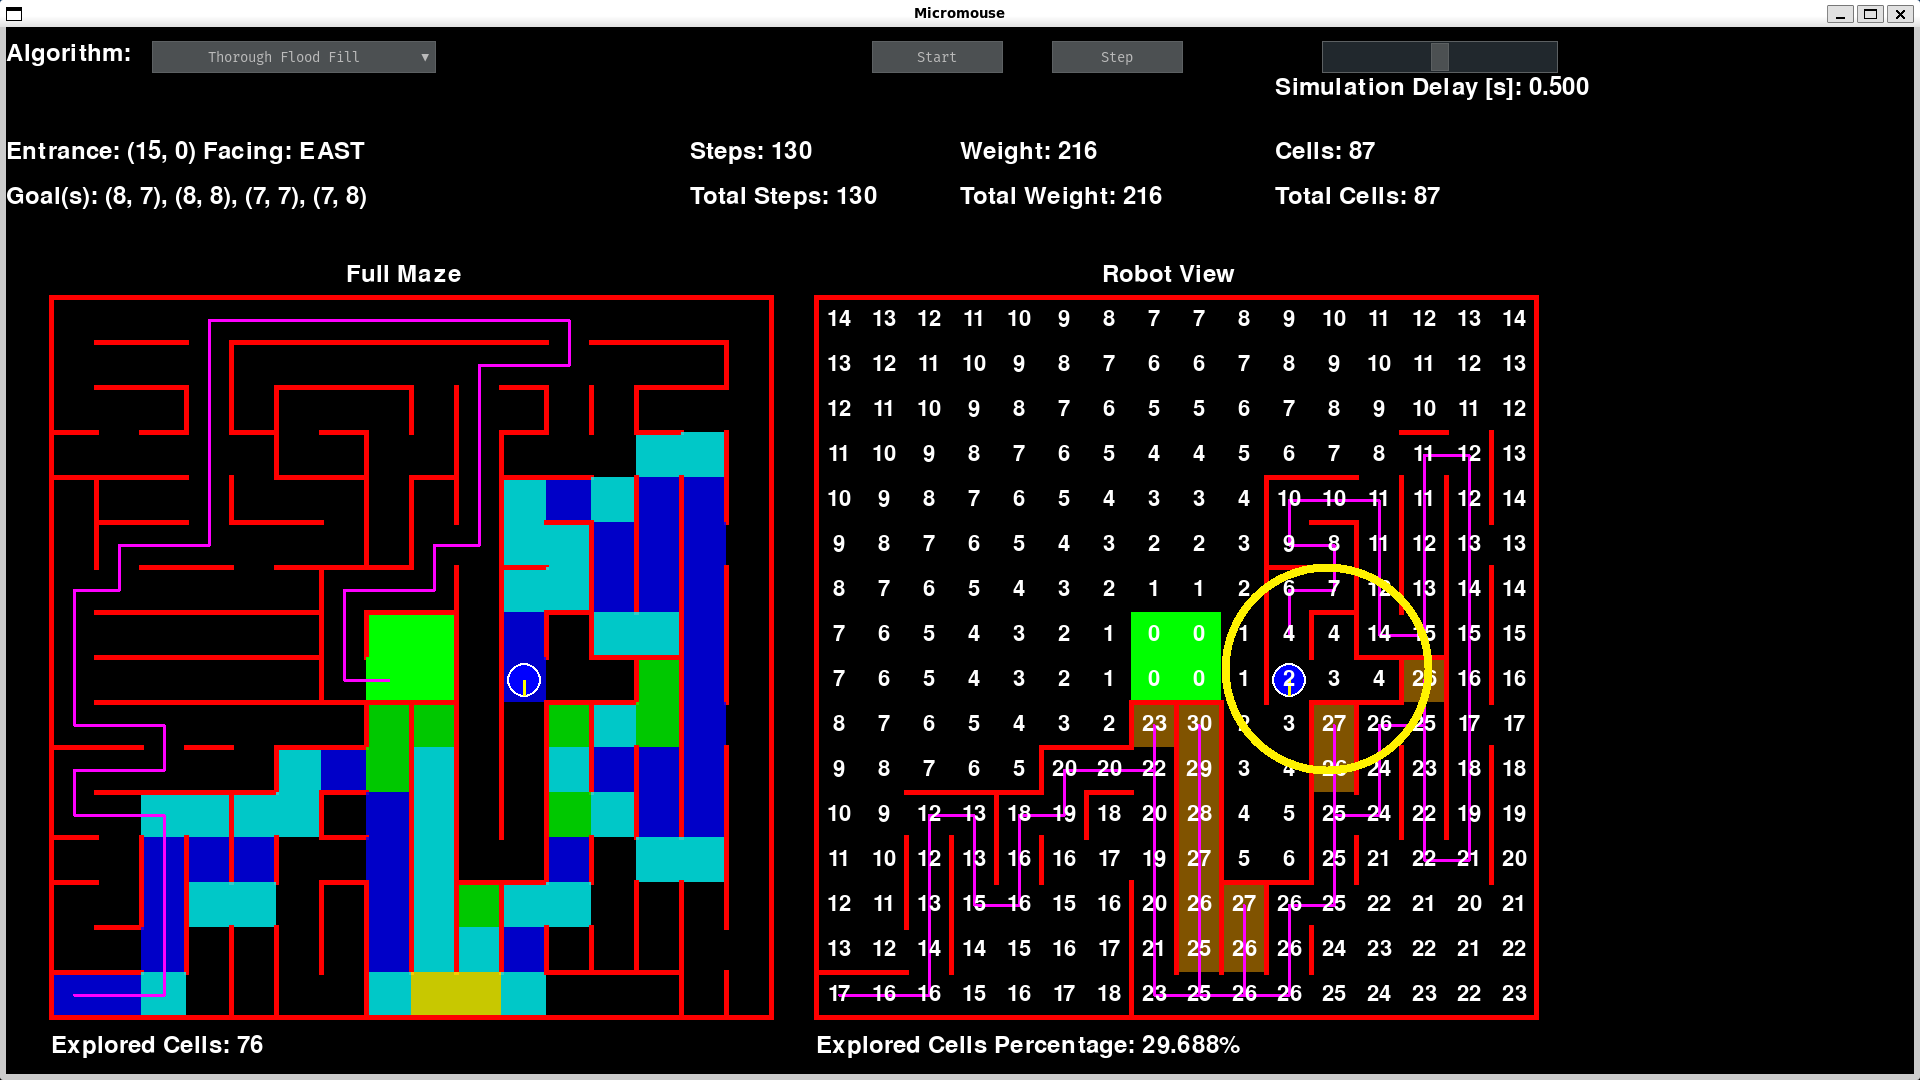
\includegraphics[width=\textwidth]{images/thorough_dead_end_before_c.png}
\caption{Thorough flood-fill before coloring dead-end to the right}
\label{Before dead-end detection}
\end{figure}

Figure \ref{After dead-end detection} shows the state after the robot tries to put an imaginary wall to its right and checks if any group of \gls{cell}s is disconnected from the graph.
Notice that the three \gls{cell}s mentioned above are now colored differently.
Those \gls{cell}s are marked as a dead-end, and the robot won't enter them in the future while exploring the \gls{maze} or solving it.

\begin{figure}[H]
\centering
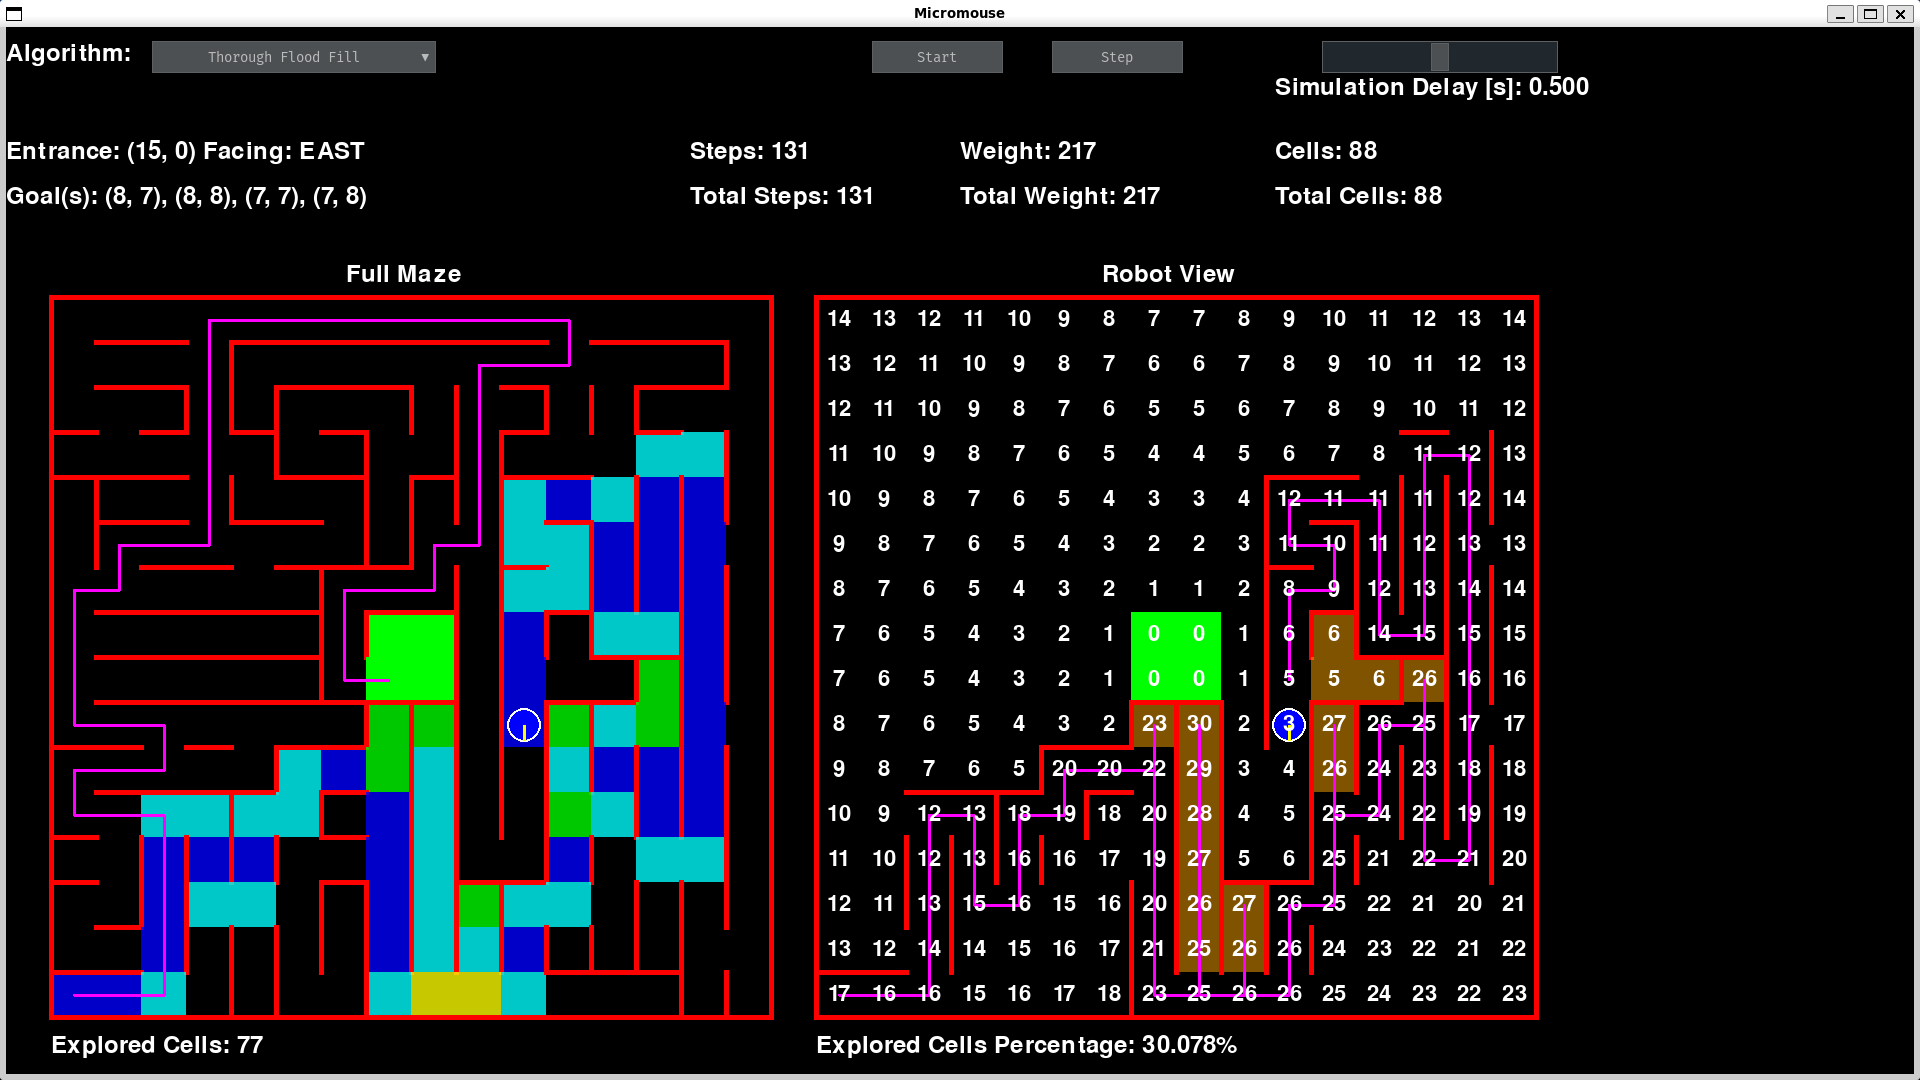
\includegraphics[width=\textwidth]{images/thorough_dead_end_after.png}
\caption{Thorough flood-fill after coloring dead-end to the right}
\label{After dead-end detection}
\end{figure}

This technique allows the robot to save time and still get all the information needed to find the fastest route to solve the \gls{maze}.

\paragraph{Flood-Fill as a Dead-End Detector}
The method mentioned above can detect dead-ends.
A dead-end is an area of the \gls{maze} with only one way in or out.
But, we also want to detect areas of the \gls{maze} that are not dead-ends but are still not worth going through.
We will refer to those areas as dead-ends even though they might have more than one way in or out.

The flood-fill dead-end detection algorithm works by looking at the flood-fill distances of each \gls{cell} in the \gls{maze} from the goal and tries to find groups of \gls{cell}s that satisfy the following criteria:
\begin{itemize}
    \item Every \gls{cell} in the group must have a distance higher than the \gls{cell}s from which the robot can access the group.
    \item The group does not contain the starting \gls{cell} or the goal \gls{cell}s.
\end{itemize}
Such groups are guaranteed to not be part of the shortest path according to the flood-fill algorithm.

Every time the robot gains new information about the \gls{maze}, the flood-fill distances are re-calculated, and if a group of \gls{cell}s satisfies the conditions above, it is considered a dead-end.

For example, in figure \ref{Before dead-end detection using flood-fill}, the robot is making its way to a \gls{cell} while exploring the \gls{maze}.
Notice the group of \gls{cell}s the robot is facing.
The region of interest is marked on the image with a circle.
Those \gls{cell}s are making a detour around the main path. Therefore, they are not worth checking.
In this position, the robot knows about all the walls surrounding this group of \gls{cell}s.

\begin{figure}[H]
\centering
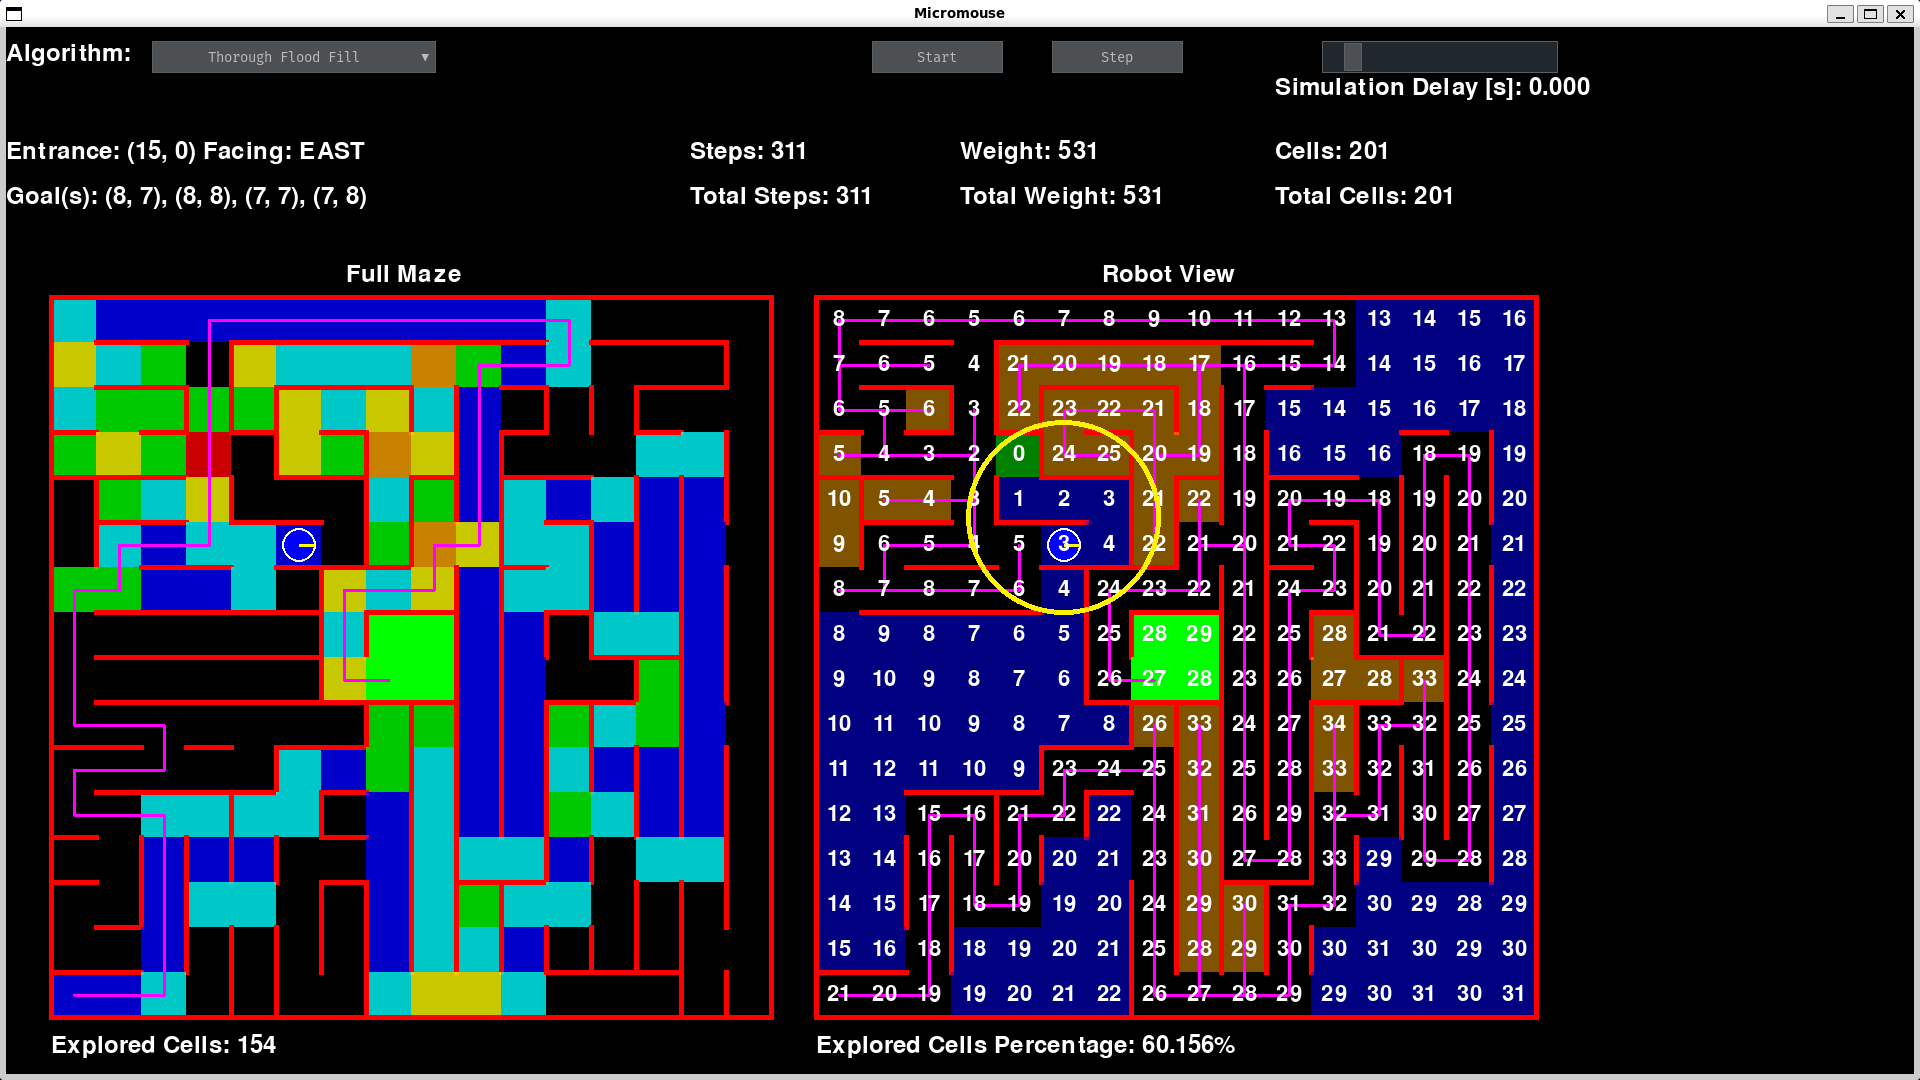
\includegraphics[width=\textwidth]{images/thorough_ff_de_before_c.png}
\caption{Thorough flood-fill before coloring dead-end using flood-fill}
\label{Before dead-end detection using flood-fill}
\end{figure}

Figure \ref{After dead-end detection using flood-fill} shows the state after the robot updated the flood-fill distances of the \gls{maze} and found the group of \gls{cell}s that satisfy the dead-end conditions.
Those \gls{cell}s are now a dead-end, and the robot won't get into them in the future while exploring the \gls{maze} or solving it.
Moreover, notice that the target \gls{cell} the robot was trying to go to is now marked as explored, and the robot changed its exploration target.

\begin{figure}[H]
\centering
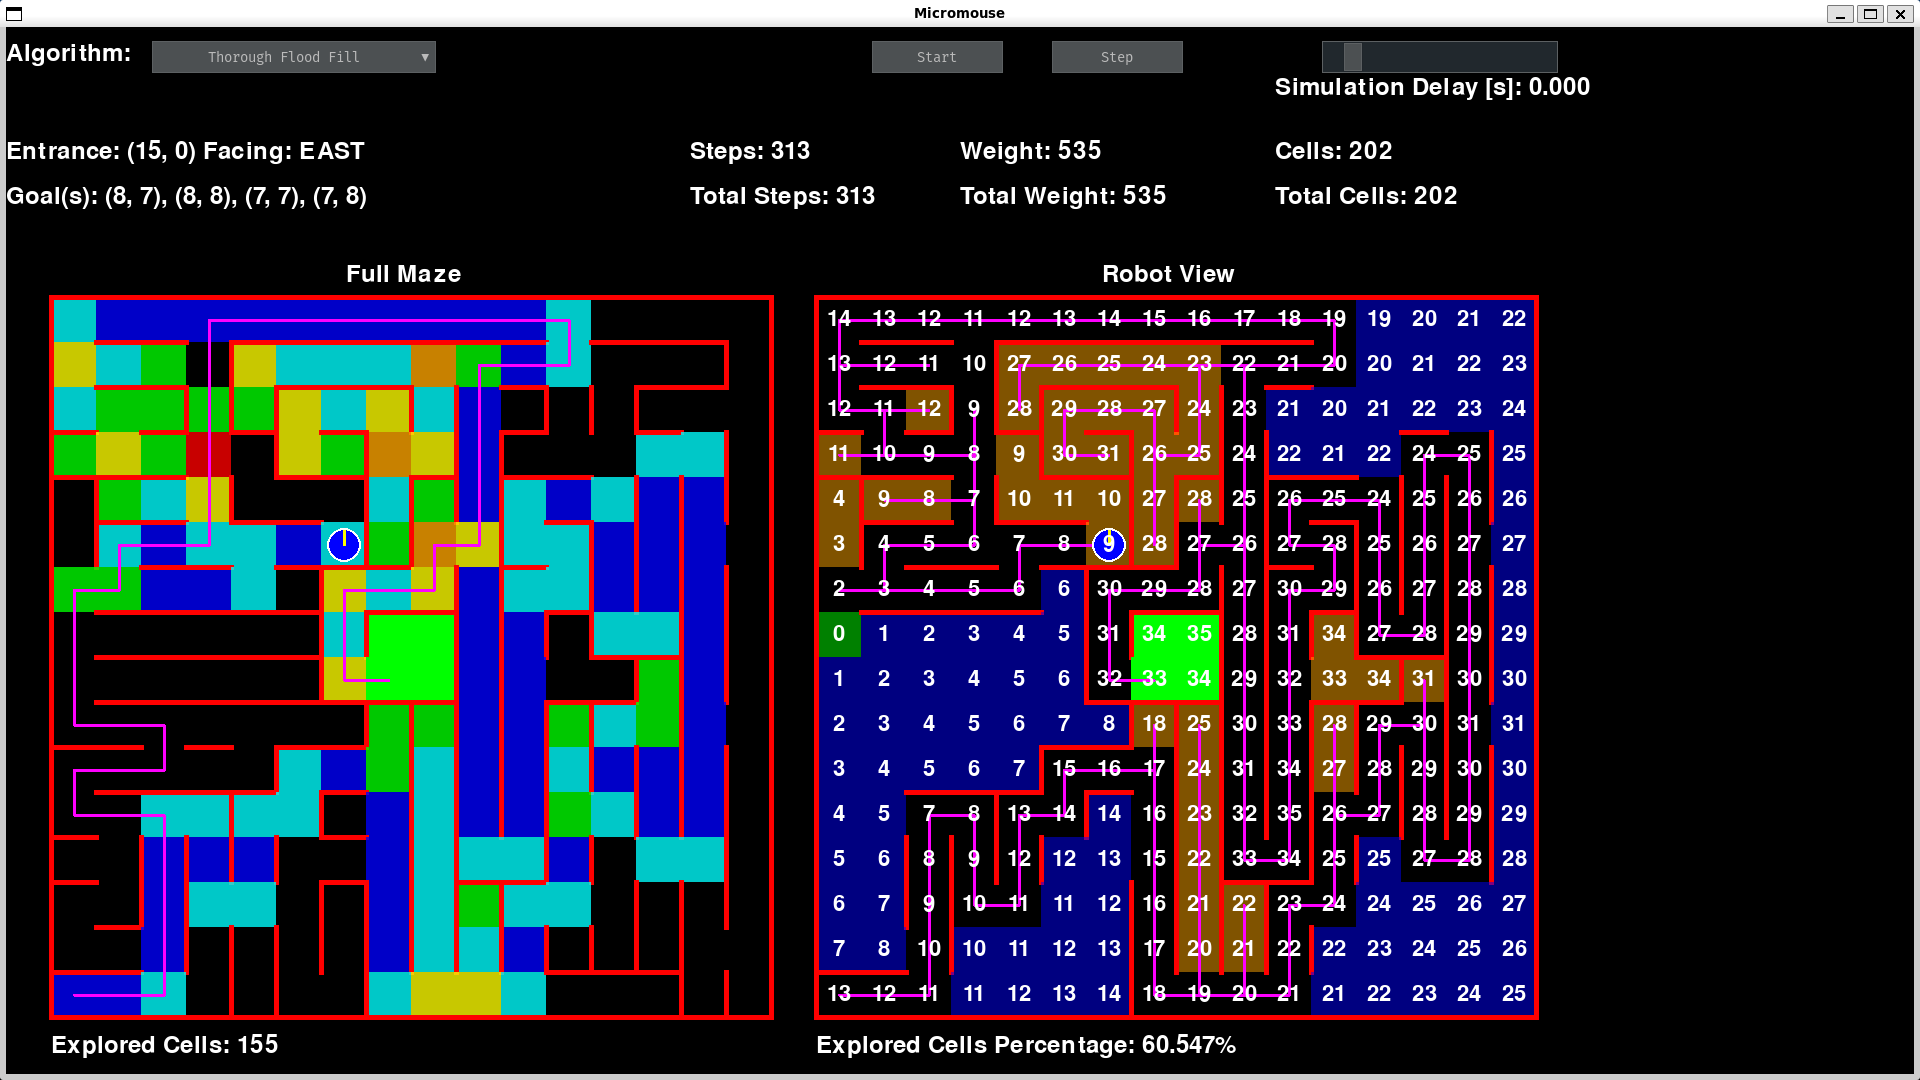
\includegraphics[width=\textwidth]{images/thorough_ff_de_after.png}
\caption{Thorough flood-fill after coloring dead-end using flood-fill}
\label{After dead-end detection using flood-fill}
\end{figure}

The problem with this approach is that the flood-fill algorithm uses distance from the goal as its weight function.
As explained earlier, in section \ref{Flood-fill drawbacks}, the flood-fill algorithm finds the shortest path and not the fastest one, which we seek.
This property means that in some cases, the flood-fill dead-end detection algorithm might find a section of the \gls{maze} not worth a visit and mark it as a dead-end even though it is part of the fastest path (but not the shortest).
Therefore, Dijkstra's algorithm is run every time this algorithm finds a dead-end to check if the fastest path goes through a group of \gls{cell}s marked as a dead-end.
If the fastest path goes through such a group, this group is then removed from the dead-end list and is re-added to the unexplored \gls{cell}s groups.

The flood-fill dead-end detection algorithm was tested with the \gls{maze} from the Japan 2017 \gls{Micromouse} competition (The \gls{maze} appears in the explanation video mentioned in section \ref{explanation video} at 10 minutes and 30 seconds into the video).
A thorough flood-fill explorer with flood-fill dead-end detection "competed" against an identical robot without flood-fill dead-end detection.
Both robots found the optimal route.
However, the exploration phase was different.
Table \ref{flood-fill dead-end detection table} shows the number of actions each robot made during the exploration phase, the weight of those actions calculated by the time weights defined in section \ref{Maze as a Directed Weighted Graph}, and the number of \gls{cell}s each robot went through.

\begin{table}[H]
    \centering
    \begin{tabular}{ | l | c | c | c | }
    \hline
        Flood-Fill Dead-End Detection & Steps & Weight & Cells \\
    \hline
         Off & 762 & 1312 & 484 \\
    \hline
         On & 612 & 1042 & 394 \\
    \hline
         \textit{Improvement} & 24.51\% & 25.91\% & 22.84\% \\
    \hline
    \end{tabular}
    \caption{Flood-fill dead-end detection comparison}
    \label{flood-fill dead-end detection table}
\end{table}

The improvement is defined to be the percentage error between the "on" and "off" values using the following formula:
$$Improvement = \frac{\textrm{Off}-\textrm{On}}{\textrm{Off}} \cdot 100\%$$

\paragraph{Conclusion}
Using the two methods above to detect dead-ends can significantly improve the exploration time while still exploring enough of the \gls{maze} to find the fastest route in any \gls{maze}.

\subsubsection{Drawbacks}
\paragraph{}
This solution solves the problem presented in section \ref{Combining Flood-Fill with Dijkstra's Algorithm} and finds the fastest route with higher probability.
Although the algorithm takes longer to explore the \gls{maze}, it tries to do so efficiently.

\section{Results and Conclusions} \label{results}
\subsection{Results Evaluation}
\paragraph{}
The Chinese 2009 \gls{IEEE} \gls{Micromouse} competition semifinal \gls{maze} was used to evaluate the results.
The \gls{maze} can be seen in figure \ref{Simulation screen} in the full \gls{maze} view (left) with the optimal solution in terms of the time weights as defined in section \ref{Maze as a Directed Weighted Graph}.
Each algorithm was evaluated by the number of actions the robot made during the exploration phase and the solution, and the weight of the solution path by the time weights defined in section \ref{Maze as a Directed Weighted Graph}.
Table \ref{Results table} presents the results of each algorithm solving the \gls{maze}.

Because the algorithms were tested in a simulation, measuring the time of running the algorithm, which is the scoring criterion in the \gls{Micromouse} competition, has less meaning.
We assume all algorithms use the same "physical" robot.
Therefore, the time it takes an algorithm to solve the \gls{maze} is defined only by the actions it issues the robot.

The results include a comparison between the flood-fill algorithm described in section \ref{Flood-Fill Algorithm}, the flood-fill with Dijkstra algorithm described in section \ref{Combining Flood-Fill with Dijkstra's Algorithm}, and the thorough flood-fill algorithm described in section \ref{thorough flood-fill algorithm}.
The results do not include algorithms described in section \ref{naive-algorithms} because they either can not solve the \gls{maze} or do it in a reasonable time.

\begin{table}[H]
    \centering
    \begin{tabular}{ | m{4cm} | c | c | c | }
    \hline
        Algorithm & Flood-Fill & Flood-Fill with Dijkstra & Thorough Flood-Fill \\
    \hline
         Number of Actions for Exploring & 300 & 300 & 619 \\
    \hline
         Number of Actions for Solution & 83 & 81 & 69 \\
    \hline
         Solution Weight & 130 & 128 & 108 \\
    \hline
    \end{tabular}
    \caption{Comparison between algorithms}
    \label{Results table}
\end{table}

\subsection{Result Explanation}
\paragraph{}
Both the flood-fill algorithm and the "flood-fill with Dijkstra" algorithm have the same exploration method.
The "flood-fill with Dijkstra" algorithm achieved a better solution than the flood-fill algorithm alone because it tried to find the fastest route rather than the shortest one.
The "flood-fill with Dijkstra" algorithm does not continue to explore the \gls{maze} and applies Dijkstra's algorithm on the \gls{maze} as it is after the flood-fill algorithm.
The explored \gls{maze} lacks the information needed to find the optimal solution with Dijkstra's algorithm.
The thorough flood-fill algorithm makes sure the information needed to find the optimal solution is available and thus has successfully found the fastest route.
The trade-off of the thorough flood-fill algorithm is the longer exploration time portrayed by more actions for exploring the \gls{maze}.

\subsection{Conclusions}
\paragraph{}
In different \gls{maze}s, both the flood-fill and flood-fill with Dijkstra algorithms may yield different results where one is better than the other or both give the same results.
The fluctuation is because our implementation of the flood-fill algorithm allows the robot to continue and explore the \gls{maze} on its second run when trying to reach the goal after the initial run exploring the \gls{maze}.
Meaning the robot can step in unexplored \gls{cell}s.
The flood-fill with Dijkstra's algorithm does not allow the robot to visit new \gls{cell}s on its second run and relies solely on the \gls{cell}s explored during the first run.
But, if exploration time is less of a concern, then using the thorough flood-fill algorithm can yield the fastest route by the given time weights in any \gls{maze}.

\subsection{Other Possible Solutions}
\subsubsection{Partition-Center Algorithm}
\paragraph{}
Another possible solution is the \textit{partition-center algorithm}, which can be implemented and tested in the simulation.
This algorithm divides the \gls{maze} into partitions.
The robot follows a different algorithm to find the fastest path possible \cite{5497446} in each partition.

\subsubsection{Other algorithms for finding the fastest path}
\paragraph{Bellman–Ford Algorithm}
The Bellman-Ford algorithm can find the fastest path in a directed weighted \gls{graph}.
We considered using this algorithm but figured its complexity was very high compared to Dijkstra's algorithm.
The complexity of this algorithm is given by $O(|V||E|)$ where $|V|$ is the number of vertices in the \gls{graph} and $|E|$ is the number of edges in the \gls{graph}.
The primary difference to Dijkstra's algorithm is that the Bellman-Ford algorithm can detect negative-weight circles in the \gls{graph}.
However, negative weights don't make sense for time-based weights.

\paragraph{Johnson's Algorithm}
Johnson's algorithm is another algorithm to find the fastest path in a directed weighted \gls{graph}.
We considered using this algorithm but figured its complexity was very high.
The complexity of this algorithm is given by $O(|V|^2\log |V| + |V||E|)$ where $|V|$ is the number of vertices in the \gls{graph} and $|E|$ is the number of edges in the \gls{graph}.
Moreover, this algorithm finds the fastest path between all pairs of vertices in the \gls{graph}, meaning between every two \gls{cell}s in the \gls{maze}.
However, we only care about paths from the starting \gls{cell}, meaning this algorithm does redundant work.

\paragraph{}
When the robot has no information about the \gls{maze}, using any of the mentioned algorithms might help navigate the \gls{maze}.
But, every time the robot gains new information about the \gls{maze}, it must repeat the algorithm to account for the change in the \gls{maze}.
The high complexity of those algorithms makes them less viable candidates for exploring and solving the \gls{maze}.
But, further research can validate this point.

\subsection{Future Research}
\subsubsection{Diagonals}
\paragraph{}
Our simulation only supports rotation in a 90\textdegree\ resolution.
This limitation does not allow the robot to move freely in the \gls{maze} as possible in a real \gls{Micromouse} \gls{maze}.
Implementing support for rotations in other degrees, such as 45\textdegree\ rotations, will allow the robot to move diagonally across the \gls{maze}.
Supporting diagonal movement will require changing the implementation of the algorithms described in this paper to include such movements.
Allowing the robot to move in diagonals or more freely can further improve the solving time and allow for a faster path in some cases.

\subsubsection{Improve Thorough Flood-Fill Exploring}
\paragraph{}
The thorough flood-fill algorithm exploring time is greatly affected by the route chosen for exploring.
If the destination \gls{cell}s for exploring are chosen in a way the robot is traveling across \gls{cell}s already explored multiple times, the exploration time can grow drastically.
Our solution takes the \gls{cell} that is furthest away from the current \gls{cell} and is part of the largest group of unexplored \gls{cell}s as the exploration goal, as described in section \ref{thorough flood-fill algorithm}.
This method can lead to the robot going back and forth across the \gls{maze} and spending precious time doing so.
It is possible that the best exploration method depends on the \gls{maze} structure and might change from one \gls{maze} to another.

\subsubsection{Optimizing the Maze Representation}
\paragraph{}
Our \gls{maze} representation uses the "maz" format covered in section \ref{maz-format}.
As seen in table \ref{maz format cell memory}, only the lower \gls{nibble} is used.
A more efficient \gls{maze} representation can hold the information about the presence of walls of two \gls{cell}s in a single byte to save memory.
Another possible way to optimize memory usage is saving data about the current \gls{cell} in the high \gls{nibble}, such as color, whether the \gls{cell} was visited, and so on.
The downside might be more computations and higher complexity to extract the data from the relevant bits.

\subsubsection{Channels}
\paragraph{}
Channels are sections of the \gls{maze} where the robot can only move forward.
The flood-fill algorithm can be optimized to perform fewer calculations when the robot is inside a channel.
Although this improvement will not improve the number of actions the robot takes, it can improve the efficiency of the flood-fill algorithm, which, in turn, can improve the time it takes for the robot to solve the \gls{maze} \cite{5591159}.

\subsubsection{Testing in a Real Environment}
\paragraph{}
Although the simulation is an easy testing tool for \gls{Micromouse} solving algorithms, nothing compares to a real robot in a real \gls{maze}.
Our new proposed algorithm, Thorough Flood-Fill, described in section \ref{thorough flood-fill algorithm}, has not been tested on a real machine.
Testing the algorithm in a physical environment requires facing the mechanical challenge as well as the algorithmic one.

\newpage

\section{Appendix}
\subsection{Project's Code} \label{Project Repo}
\paragraph{}
The source code, installation instructions, and more are found on GitHub at the following link: \url{https://github.com/Roynecro97/micromouse-py-sim}.

\begin{center}
\qrcode[height=1in]{https://github.com/Roynecro97/micromouse-py-sim}
\end{center}

\subsection{Running The Simulation}
\subsubsection{Code Installation}
\paragraph{}
\begin{enumerate}
    \item Clone the repository:
    \begin{verbatim}
    git clone https://github.com/Roynecro97/micromouse-py-sim &&
    cd micromouse-py-sim
    \end{verbatim}
    \item Create a \textit{virtualenv} (optional):
    \begin{verbatim}
    python3.12 -m virtualenv .venv
    source .venv/bin/activate
    \end{verbatim}
    \item Install all dev requirements:
    \begin{verbatim}
    pip install -r dev-requirements.txt
    \end{verbatim}
\end{enumerate}

\subsubsection{Running}
\paragraph{}
With the simulation installed, the \textit{micromouse} command is automatically added to the path:
\begin{verbatim}
$ micromouse -h
usage: micromouse [-h] {sim,tool} ...

Micromouse simulator.

options:
-h, --help  show this help message and exit

subcommands:
  {sim,tool}
    sim       Run the simulator.
    tool      Run a tool.
\end{verbatim}

Use the \textit{micromouse sim} command to run the simulator.
For example, from the git clone's directory, run:
\begin{verbatim}
$ micromouse sim -p semifinal
\end{verbatim}

\subsubsection{More Information}
\paragraph{}
More information about using the simulation can be found in the link provided in section \ref{Project Repo}.

\subsection{Micromouse Competition Rules}
\subsubsection{Introduction}
\paragraph{Competition Description}
In this competition, the participant, or team of participants, must design and build an
autonomous robotic ”mouse” capable of traversing a maze of standard dimensions from
a specified corner to its center in the shortest time possible.
\subsubsection{Participant Eligibility}
\paragraph{IEEE Membership}
All participants shall be registered IEEE student members attending the university they
identified when registering for the SAC.
\paragraph{Team Composition}
Teams shall consist of one to five participants. A team of four or five participants shall
not include more than two graduate students. A team of two or three participants shall
not include more than one graduate student. Teams consisting of individual graduate
students are not allowed. In the case of a team with more than one participant, it
should be possible to demonstrate that each participant made a significant contribution.
\paragraph{Number of Teams}
There is no limit to the number of teams that one university may register for this
competition.
\subsubsection{\texorpdfstring{\gls{Micromouse}} Robot Rules}
\paragraph{Fabrication}
The \gls{Micromouse} robot submitted by a team must be designed and built from scratch.
\paragraph{Self Containment}
The \gls{Micromouse} robot shall be self-contained (no remote controls). The robot shall not
use an energy source employing a combustion process.
\paragraph{Dislodged Parts}
The \gls{Micromouse} robot shall not separate from any part of itself while navigating the
\gls{maze}. To complete the \gls{maze}, the robot, in its entirety, must enter the center of the
\gls{maze}.
\paragraph{Method of Movement}
The \gls{Micromouse} robot shall not jump over, fly over, climb, scratch, cut, burn, mark,
damage, or destroy the \gls{maze}'s walls.
\paragraph{\gls{Micromouse} Size}
The \gls{Micromouse} robot shall not be larger either in length or in width than 25
centimeters. The dimensions of a \gls{Micromouse} robot that changes its geometry shall not
be greater than 25cm x 25cm (length and width, respectively). There are no restrictions
on the height of the robot.
\paragraph{Inspection}
All \gls{Micromouse} robots are subject to inspection before starting their competition, to
ensure they are within the specifications outlined by these rules, and that they do not
pose potential safety hazards.
\paragraph{Rules Violation}
Any violation of these rules will constitute immediate disqualification from the contest
and ineligibility for any associated prizes.
\subsubsection{Maze Specifications}
\paragraph{Maze Dimensions}
The \gls{maze} is composed of 18cm x 18cm unit squares arranged to form a 16 x 16 unit grid.
The walls of the \gls{maze} units are 5 cm high and 1.2 cm thick (assume a 5\% tolerance
for \gls{maze}s). An outside wall encloses the entire \gls{maze}.
\paragraph{Maze Coloration}
The sides of the \gls{maze} walls are white, the tops of the walls are red, and the floor is
black. The \gls{maze} is made of wood and finished with non-gloss paint.
\paragraph{Maze Fabrication Inconsistencies}
Do not assume the walls are consistently white, that the tops of the walls are
consistently red, or that the floor is consistently black. Fading may occur and
parts from different \gls{maze}s may be used. Do not assume the floor provides a
given amount of friction. It is simply painted plywood and may be quite slick. The
\gls{maze} floor may be constructed using multiple sheets of plywood. Therefore
there may be a seam between the two sheets on which any low-hanging parts of
the robot may snag.
\paragraph{Start/End Zones}
The starting square of the \gls{maze} is located at one of the four corners. The starting square
is bounded on three sides by walls. The start line is located between the first and second
squares. As the mouse exits the corner square (signified by crossing the start line), the
run timer starts. The destination is a gateway to the four-unit square at the center of the
\gls{maze}. The destination square has only one gateway.
\paragraph{Lattice Points}
Small square posts, each 1.2 cm x 1.2 cm, at the four corners of each unit square are
called lattice points. The \gls{maze} is assembled so that there is at least one wall at each
lattice point.
\paragraph{Multiple Paths}
Multiple paths from the starting square to the destination square are allowed and
should be expected. The destination square will be positioned so that a wall-hugging
mouse will NOT be able to find it.
\subsubsection{Competition Rules} \label{Competition Rules}
\paragraph{Time}
Each team is allocated 10 minutes of access to the \gls{maze}, starting when the competition
administrator acknowledges the team and grants access to the \gls{maze}. Any time used to
adjust the team’s \gls{Micromouse} robot between runs is included in these 10 minutes. A
run-time is recorded for each run (from the start cell to the center zone) in which the
robot successfully reaches the destination square. The minimum run time within the 10-minute trial
shall be the mouse’s official time.
\paragraph{Stopping/Removing the \gls{Micromouse} Robot}
Each run shall be made from the starting square. Multiple runs, or run attempts, may be
made within the allotted 10-minute \gls{maze} time. The team may abort a run at any time,
and return the \gls{Micromouse} robot to the starting square. If the robot has reached the
destination square and has acquired a “run time,” the robot may take the \gls{maze} back to
the corner starting square on its own. Alternatively, it may be removed at any time
without affecting the runtime of that run. If the robot is placed back in the \gls{maze} at the
starting square, a one-time penalty of 30 seconds will be added to the robot’s next run
time.
\paragraph{Reprogramming After Reveal}
After the competition \gls{maze} is revealed to the teams at the start, the
operator shall not reprogram his or her \gls{Micromouse} robot but may elect to change the
positions of switches on the robot.
\paragraph{Room Conditions}
The illumination, temperature, and humidity of the room shall be those of an ambient
environment. (40 to 120 degrees F, 0\% to 95\% humidity, non-condensing).
\paragraph{Ambient Lighting}
Do not make any assumptions about the amount of sunlight, incident light, or
fluorescent light that may be present at the competition site.
\paragraph{Run Time}
The run timer will start when the front edge of the \gls{Micromouse} robot crosses the start
line and stops when the front edge of the mouse crosses the finish line. The start line is
at the boundary between the starting unit square and the next unit square clockwise.
The finish line is at the entrance to the destination square.
\paragraph{Starting a Run}
A new run begins every time the \gls{Micromouse} robot leaves the starting square. If the
robot does not enter the destination square, no runtime is recorded. For example, if the
robot re-enters the starting square (before entering the destination square) on a run,
that run is aborted, and a new runtime will begin when the robot leaves the starting
square.
\paragraph{Continued Navigation}
If the \gls{Micromouse} robot continues to navigate the \gls{maze} after reaching the destination
square, the time taken will not count toward any run. The robot may and should make
several runs without being touched by the operator. Once the robot has found the
center, it is common practice to explore the \gls{maze} via an alternate path on the return
trip to the starting square.
\paragraph{Modifying the Robot}
The team may not feed information about the \gls{maze} to the \gls{Micromouse} robot.
Therefore, changing ROMs or downloading programs is NOT allowed once the \gls{maze} is
revealed. However, participants are allowed to do the following:
\begin{itemize}
\item Change switch settings (e.g. to select algorithms).
\item Replace batteries between runs.
\item Adjust sensors.
\item Change speed settings.
\item Make repairs.
\end{itemize}
\paragraph{Changing the Robot’s Weight}
After the team’s 10-minute time allotment begins, they shall not alter their \gls{Micromouse}
robot in a manner that alters its weight (e.g. removal of a bulky sensor array or
switching to lighter batteries to get better speed after mapping the \gls{maze} is not
allowed). The judges shall arbitrate all interactions with the robot.
\subsubsection{Scoring} \label{scoring}
\paragraph{Regionality and Presentation}
There is only one official IEEE \gls{Micromouse} contest each year in each area or region. All
\gls{Micromouse} robots, whether or not they have competed in previous contests, compete
on an equal basis. All robots must be presented to the judges by the original team.
\paragraph{Scoring}
First place goes to the team with the shortest official time (without the team touching
its \gls{Micromouse} robot during runs). Second prize to the team with the next shortest
time, and so on. Teams with the \gls{Micromouse} robot that does not enter the center
square will be ranked by the judges based on the following criteria:
\begin{itemize}
\item How close the robot gets to the destination square without being touched.
\item Evidence that the mouse knows where it is relative to the destination square.
\end{itemize}
If, on occasion, the robot becomes immobilized in a corner or on a wall, the team may
manually intervene to correct the problem (with care not to modify the mouse’s
intended direction of movement. The frequency of such corrections will be considered
by the judges while scoring.
\paragraph{Requesting Breaks}
If requested, a break may be provided to the team after the completion of a run if
another team is waiting to compete. The 10-minute timer will stop. When the team
resumes their play, the 10-minute timer will continue. Judges and administrators shall
determine whether breaks are allowed on a case-by-case basis.
\paragraph{Judges’ Discretion}
The judges reserve the right to ask the team for an explanation of their \gls{Micromouse}
robot and its actions. The judges also reserve the right to stop a run, declare
disqualification, or give instructions as appropriate (e.g., if the \gls{maze}'s structure is jeopardized by the mouse's continuing operation).

\subsection{Explanation Video About The Competition} \label{explanation video}
\paragraph{}
An informative video about the \gls{Micromouse} competition made by \textit{Veritasium} can be seen at \url{https://www.youtube.com/watch?v=ZMQbHMgK2rw}.
This video can help visualize some of the algorithms discussed in this paper and gives additional info about the mechanical aspect of the challenge, which was not discussed in this work.

\newpage

\bibliographystyle{plain}
\bibliography{refs}

\end{document}
